%%% ====================================================================
%%% Início da parte textual do documento.


%%% Configuração do espaçamento entre títulos e texto
\setlength{\afterchapskip}{1.5cm minus \baselineskip}


\chapter{Resultados}
\label{cha:resultados}

Esse capítulo contém os resultados da aplicação e dos estudos de casos aplicados.

\section{Aplicação}

\subsection{Diagrama de Classes}

Com auxílio da ferramenta \textit{Astah Community}, foi desenvolvido o seguinte Diagrama de Classes, apresentado na figura \ref{fig:diagramaClasses}:

\begin{figure}[H]
	\centering
	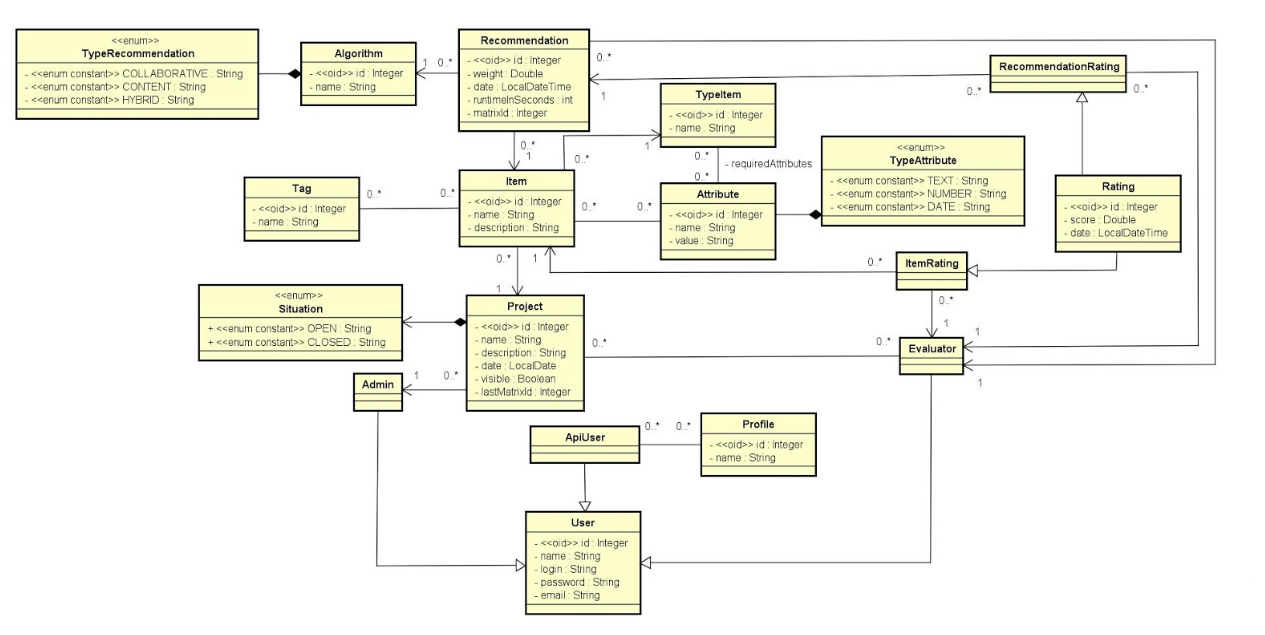
\includegraphics[width=1\linewidth]{imagens/diagramaClasses.PNG}
	\caption[Diagrama de Classes]{Diagrama de Classes}
    \label{fig:diagramaClasses}
\end{figure}

\subsection{API de Recomendação}

Foi desenvolvido uma aplicação backend aberta para uso e modificações. O código fonte de aplicação está disponível no \href{https://github.com/herikLorencao/srh-backend}{GitHub} \footnote{Link do repositório: https://github.com/herikLorencao/srh-backend} podendo ser modificado e adaptado.

Foram desenvolvidos um total de 103 endpoints para a API, que incluem desde cadastros até rotinas de autenticação e recomendação. Todas as rotas estão documentadas e disponíveis no serviço \href{https://documenter.getpostman.com/view/6420672/T1LVA4ST}{Postman} \footnote{Link dos endpoints da API: https://documenter.getpostman.com/view/6420672/T1LVA4ST} para acesso.

Na figura \ref{fig:requisicaoPostman} é possível verificar a documentação das requisições que encontra-se aberta para consulta e uso.

\begin{figure}[H]
	\centering
	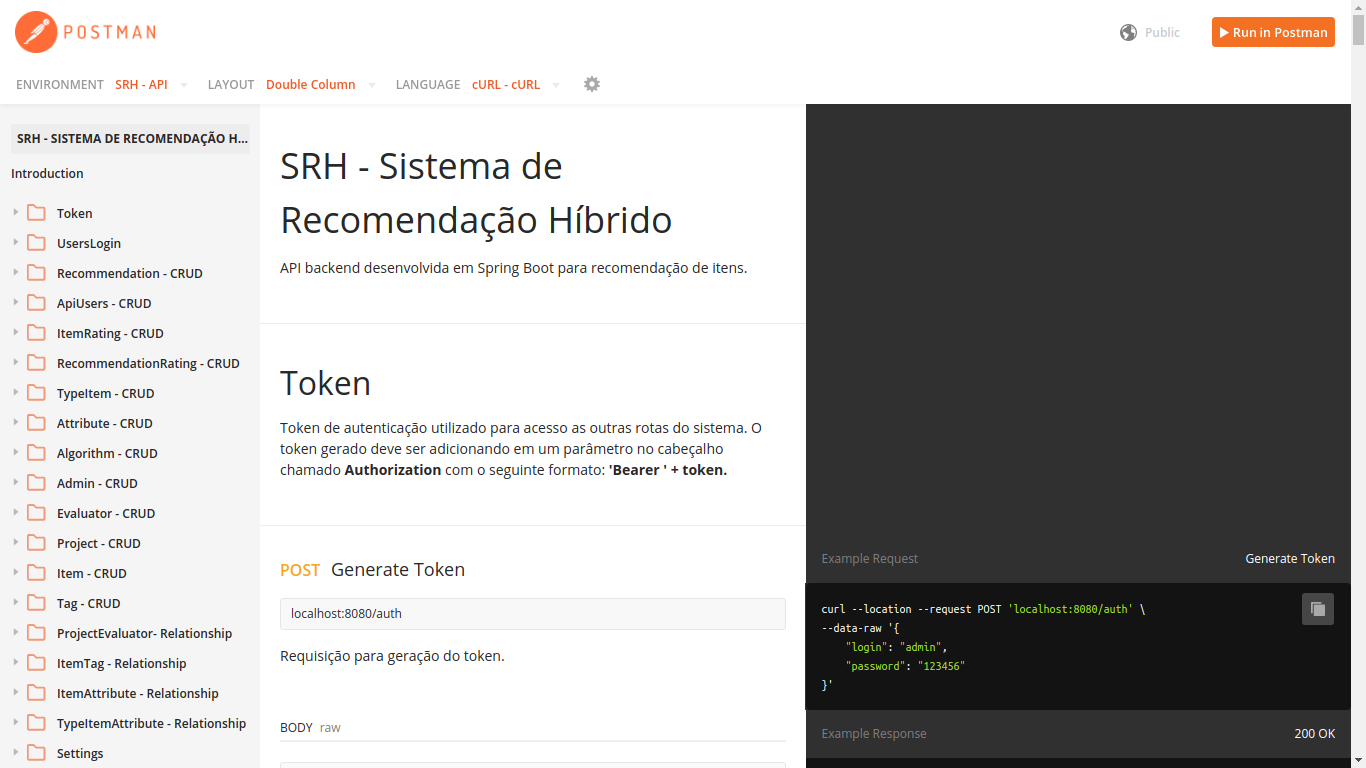
\includegraphics[width=1\linewidth]{imagens/requisicoesPostman.png}
	\caption[Documentação das requisições]{Documentação das requisições}
    \label{fig:requisicaoPostman}
\end{figure}

A API desenvolvida apresenta configuração para uso e distribuição de informação entre diversos clientes, possuindo configurações para tokenização de endpoints e criação de níveis de usuário com privilégios distintos, permitindo um maior controle de acessos aos dados e recursos do sistema.

\textbf{Concorrência}

Foi desenvolvido um endpoint que possibilita o cálculo das recomendações de maneira concorrente, a partir do uso de funções assíncronas no framework \textbf{Spring Boot}.

Como base para desenvolvimento foi utilizado o projeto oferecido pela documentação do \textbf{Spring} \footnote{Disponível em: https://spring.io/guides/gs/async-method/} que demonstra o uso do sistema de concorrência e como essa técnica pode permitir a melhoria no tempo de execução de códigos complexos.

Para os testes de velocidade, foi utilizado o seguinte ambiente para execução, mostrado na tabela abaixo:

\begin{table}[H]
\centering
\begin{tabular}{|c|c|}
\hline
\textbf{Informações} & \textbf{Tempo de Execução (ms)} \\ \hline
Número Processadores & 2                               \\ \hline
Número de Threads    & 4                               \\ \hline
Mémoria RAM          & 8 GB                            \\ \hline
Armazenamento        & 1 TB HDD                        \\ \hline
\end{tabular}
\end{table}

Com os ambientes definidos, foram executadas três requisições para cada abordagem de recomendação nos servidores onde foi mapeado o tempo de resposta para o cliente de cada recomendação. Com os dados definidos, foi realizada uma média aritmética dos valores, resultando nos seguintes dados:

\begin{table}[H]
\centering
\begin{tabular}{|c|c|}
\hline
\multicolumn{2}{|c|}{\textbf{Tempo de Recomendação - Sem Concorrência}} \\ \hline
\textbf{Informações}                 & \textbf{Tempo de Execução (s)}    \\ \hline
Recomendação Colaborativa            & 2,88                               \\ \hline
Recomendação Baseada em Conteúdo     & 3,02                               \\ \hline
Recomendação Híbrida Ponderada       & 20,64                              \\ \hline
Recomendação Híbrida Mista           & 5,64                               \\ \hline
\end{tabular}
\end{table}

\begin{table}[H]
\centering
\begin{tabular}{|c|c|}
\hline
\multicolumn{2}{|c|}{\textbf{Tempo de Recomendação - Com Concorrência}} \\ \hline
\textbf{Informações}                 & \textbf{Tempo de Execução (s)}    \\ \hline
Recomendação Colaborativa            & 30,41                              \\ \hline
Recomendação Baseada em Conteúdo     & 26,78                               \\ \hline
Recomendação Híbrida Ponderada       & 180                              \\ \hline
Recomendação Híbrida Mista           & 32,81                              \\ \hline
\end{tabular}
\end{table}

Infelizmente, devido ao nível de complexidade do algoritmo, principalmente em relação ao acesso aos dados pelo ORM \textit{(Object Relational Mapper)} foi observado uma perca de performance significativa no uso do algoritmo de maneira concorrente.

Para um melhor resultado no processo de concorrência torna-se necessário um conhecimento mais profundo acerca do gerenciamento de processos e escalonamento embutido no Spring, além de ajustes na arquitetura e modelagem do sistema procurando separar logicamente as lógicas de concorrência do restante do projeto.

\textbf{Matriz de recomendação offline}

Como forma de buscar um maneira de acesso mais rápido as recomendações, foi desenvolvido um endpoint para recomendação offline que acaba utilizando-se de dados salvos posteriormente para busca das recomendações, evitando o processamento e cálculo das recomendações novamente, o que acaba por oferecer um menor tempo de resposta para os usuários.

Vale ressaltar que esse processo utiliza-se das recomendações já salvas no banco de dados da aplicação, fazendo com que esses dados não sejam os mais atuais possíveis. Esse fator negativo é recompensado pelo menor tempo de resposta do servidor, além da redução de processamento e acesso ao banco de dados pelo sistema.

Para realização dos testes de performance, foram utilizados os mesmos ambientes de teste informados na seção de resultados relativa à concorrência. O processo de mapeamento dos dados foi semelhante, capturando o tempo de resposta das requisições e realizando a média aritmética dos resultados.

Desse modo, foi possível definir os seguintes dados:

\begin{table}[H]
\centering
\begin{tabular}{|c|c|}
\hline
\multicolumn{2}{|c|}{\textbf{Tempo de Recomendação - Sem Matriz Offline}} \\ \hline
\textbf{Informações}                 & \textbf{Tempo de Execução (s)}    \\ \hline
Recomendação Colaborativa            & 2,88                               \\ \hline
Recomendação Baseada em Conteúdo     & 3,02                               \\ \hline
Recomendação Híbrida Ponderada       & 20,64                              \\ \hline
Recomendação Híbrida Mista           & 5,64                               \\ \hline
\end{tabular}
\end{table}

\begin{table}[H]
\centering
\begin{tabular}{|c|c|}
\hline
\multicolumn{2}{|c|}{\textbf{Tempo de Recomendação - Com Matriz Offline}} \\ \hline
\textbf{Informações}                 & \textbf{Tempo de Execução (s)}    \\ \hline
Recomendação Colaborativa            & 1,96                               \\ \hline
Recomendação Baseada em Conteúdo     & 1,60                             \\ \hline
Recomendação Híbrida Ponderada       & 1,31                               \\ \hline
Recomendação Híbrida Mista           & 1,32                               \\ \hline
\end{tabular}
\end{table}
\subsection{Cliente Administrativo}

Para acesso e manipulação dos recursos do sistema foi desenvolvido um cliente administrativo para acesso na WEB. Nele é possível cadastrar, alterar, visualizar e remover os principais recursos do sistema, permitindo que um usuário com perfil de administrador possa criar e manipular diversos projetos. Nas figuras \ref{fig:clienteAdminLogin}, \ref{fig:clienteAdminProjeto}, \ref{fig:clienteAdminCriarProjeto}, \ref{fig:clienteAdminUsuarios}, \ref{fig:clienteAdminAvaliacoes}, \ref{fig:clienteAdminRecomendacoes} e \ref{fig:clienteAdminUsuarioAPI} é possível visualizar algumas das telas do sistema.

\begin{figure}[H]
	\centering
	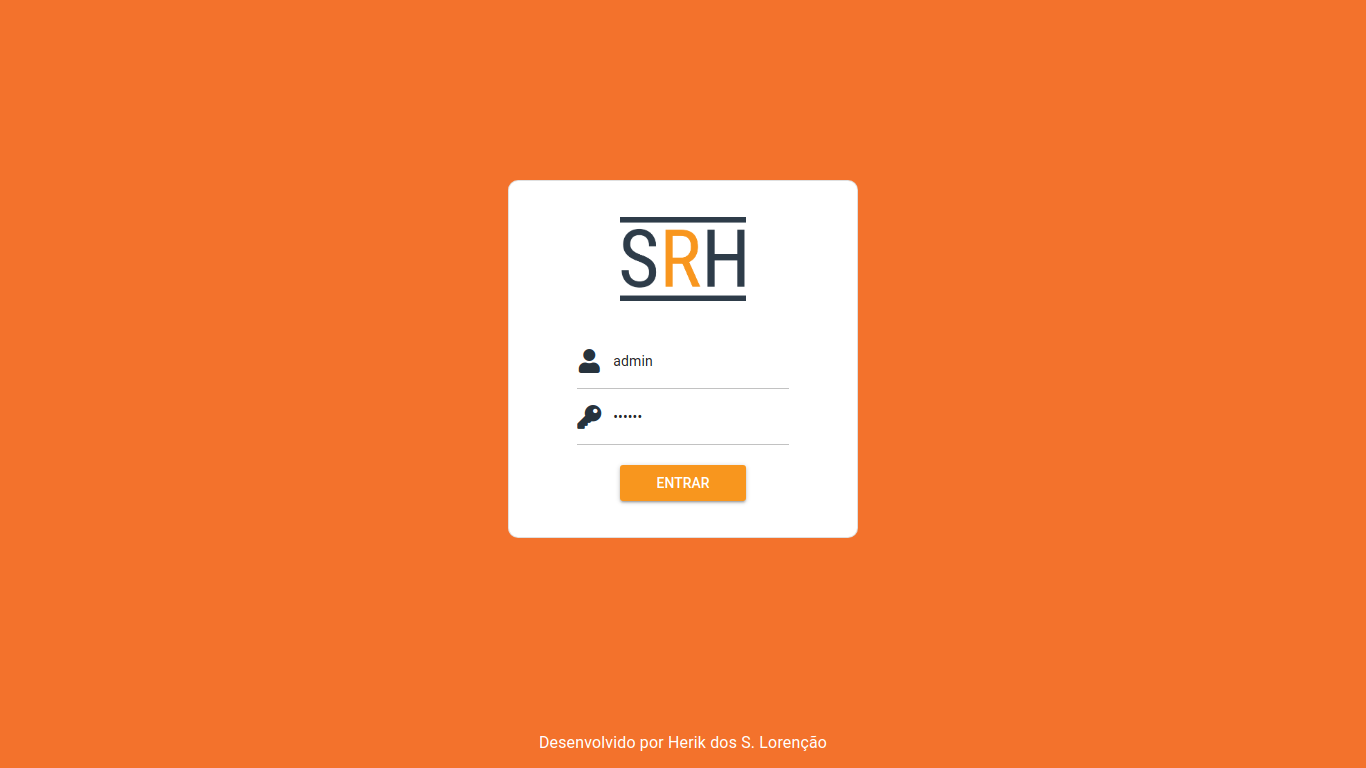
\includegraphics[width=.9\linewidth]{imagens/adminLogin.png}
	\caption[Cliente Administrativo: Login]{Cliente Administrativo: Login}
    \label{fig:clienteAdminLogin}
\end{figure}

\begin{figure}[H]
	\centering
	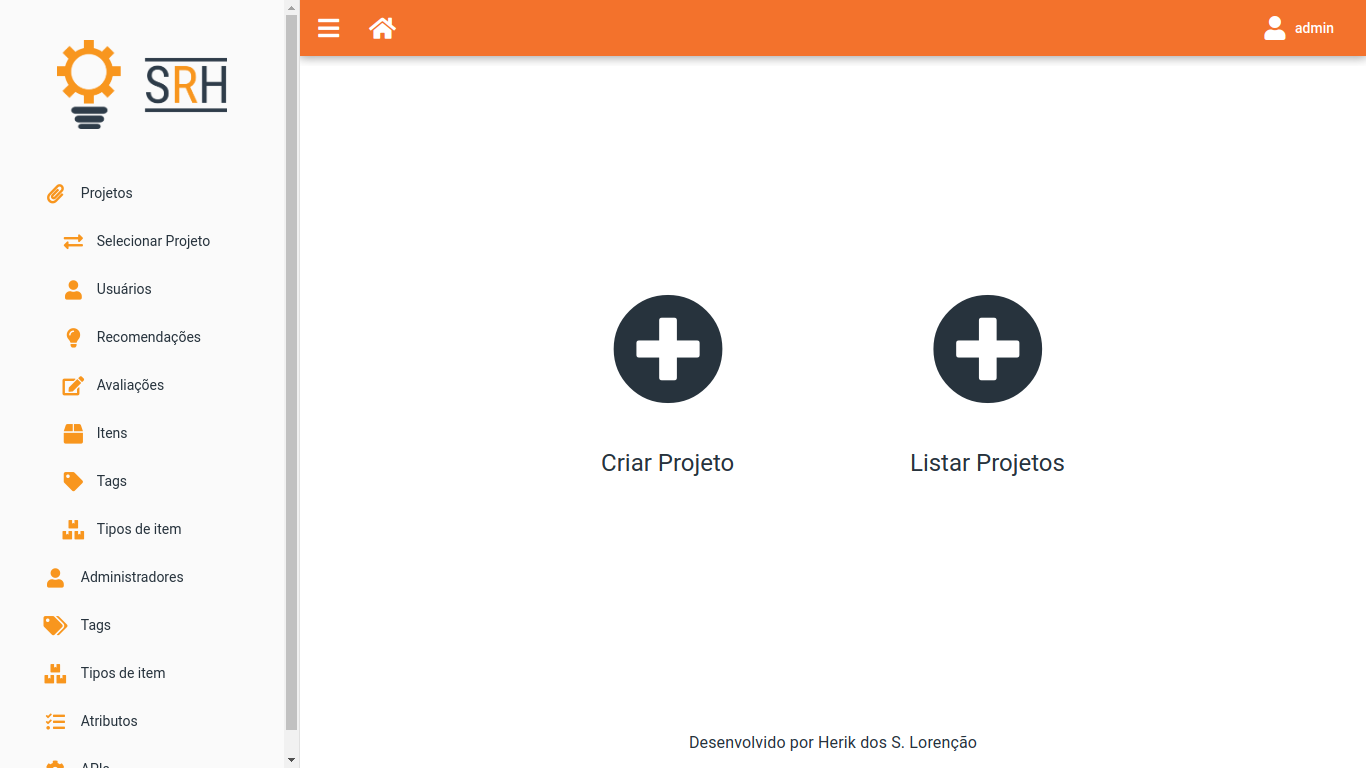
\includegraphics[width=.9\linewidth]{imagens/adminCriarProjeto.png}
	\caption[Cliente Administrativo: Projeto]{Cliente Administrativo: Projeto}
    \label{fig:clienteAdminProjeto}
\end{figure}

\begin{figure}[H]
	\centering
	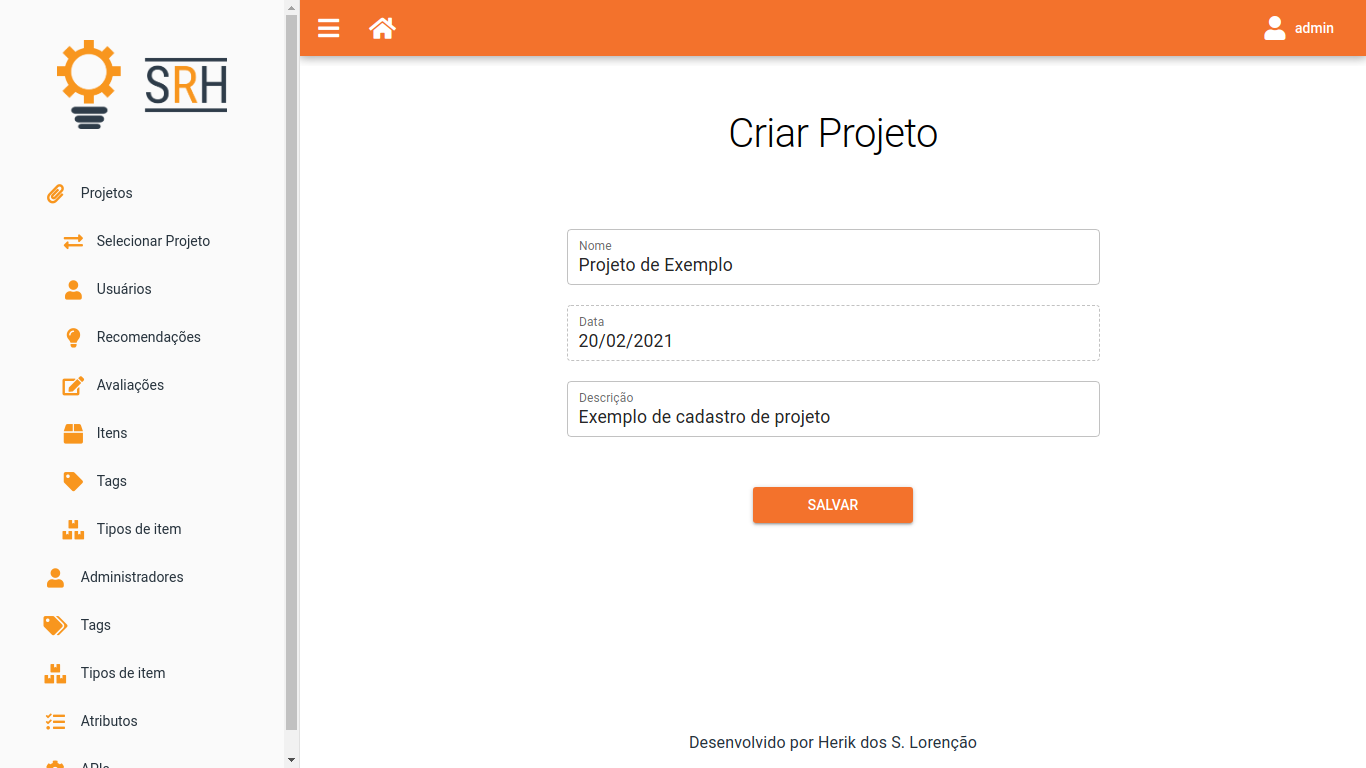
\includegraphics[width=.9\linewidth]{imagens/adminCriarProjetoForm.png}
	\caption[Cliente Administrativo: Criar Projeto]{Cliente Administrativo: Criar Projeto}
    \label{fig:clienteAdminCriarProjeto}
\end{figure}

\begin{figure}[H]
	\centering
	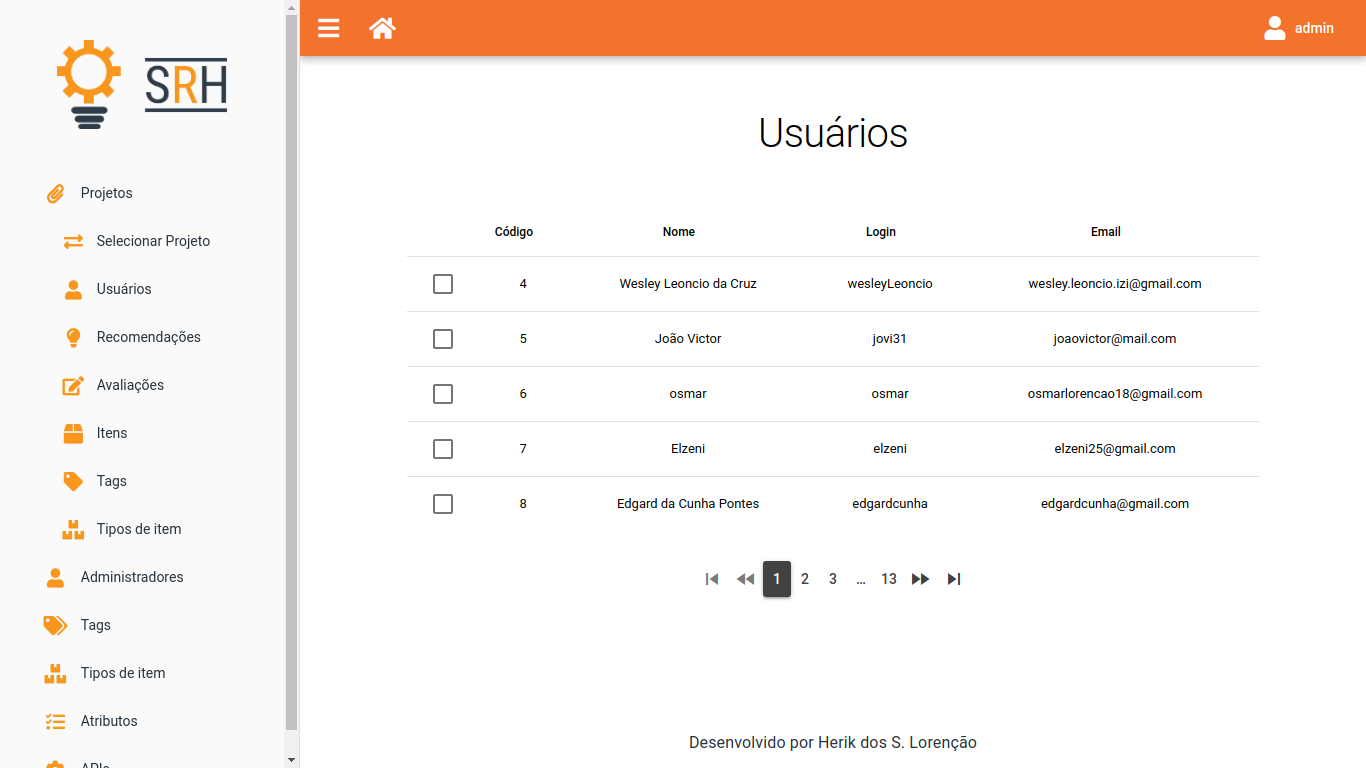
\includegraphics[width=.9\linewidth]{imagens/adminUsuarios.png}
	\caption[Cliente Administrativo - Usuários]{Cliente Administrativo: Usuários}
    \label{fig:clienteAdminUsuarios}
\end{figure}

\begin{figure}[H]
	\centering
	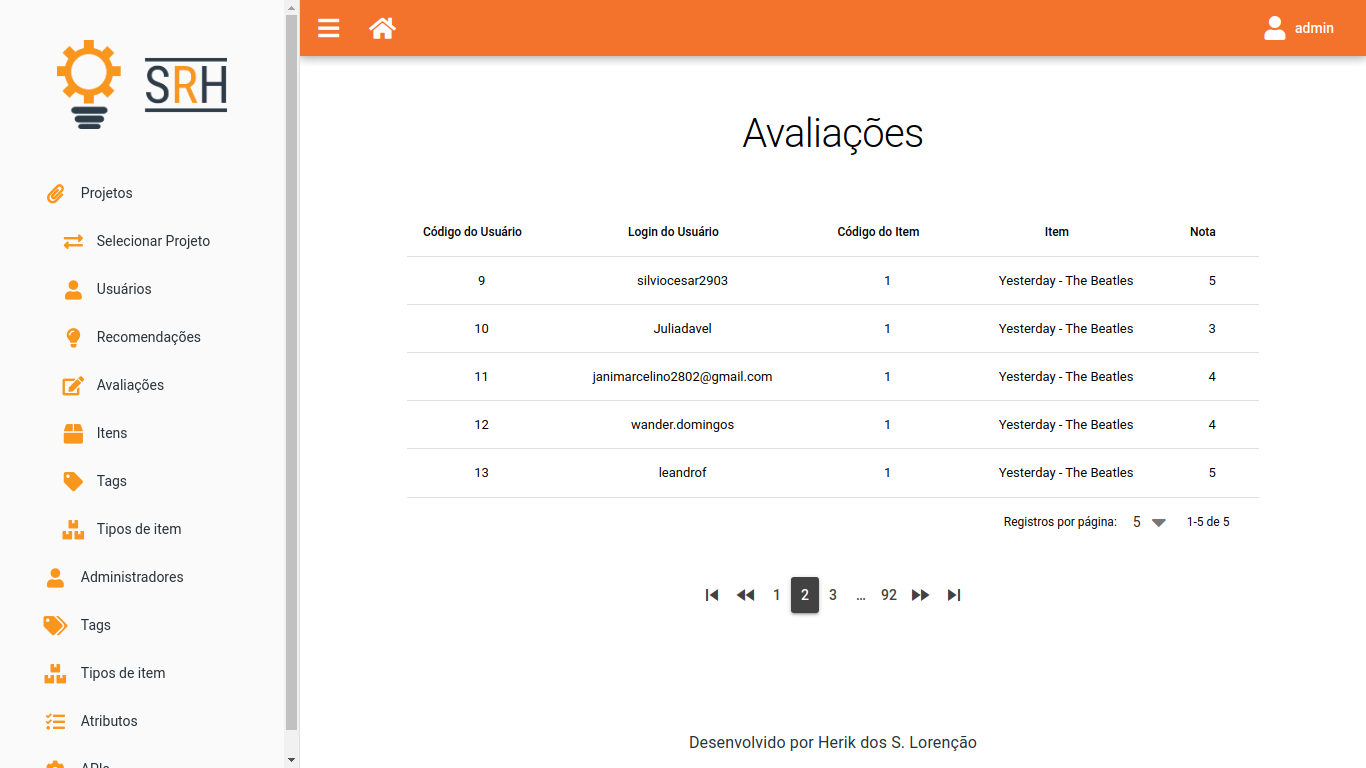
\includegraphics[width=.9\linewidth]{imagens/adminAvaliacoes.png}
	\caption[Cliente Administrativo: Avaliações]{Cliente Administrativo: Avaliações}
    \label{fig:clienteAdminAvaliacoes}
\end{figure}

\begin{figure}[H]
	\centering
	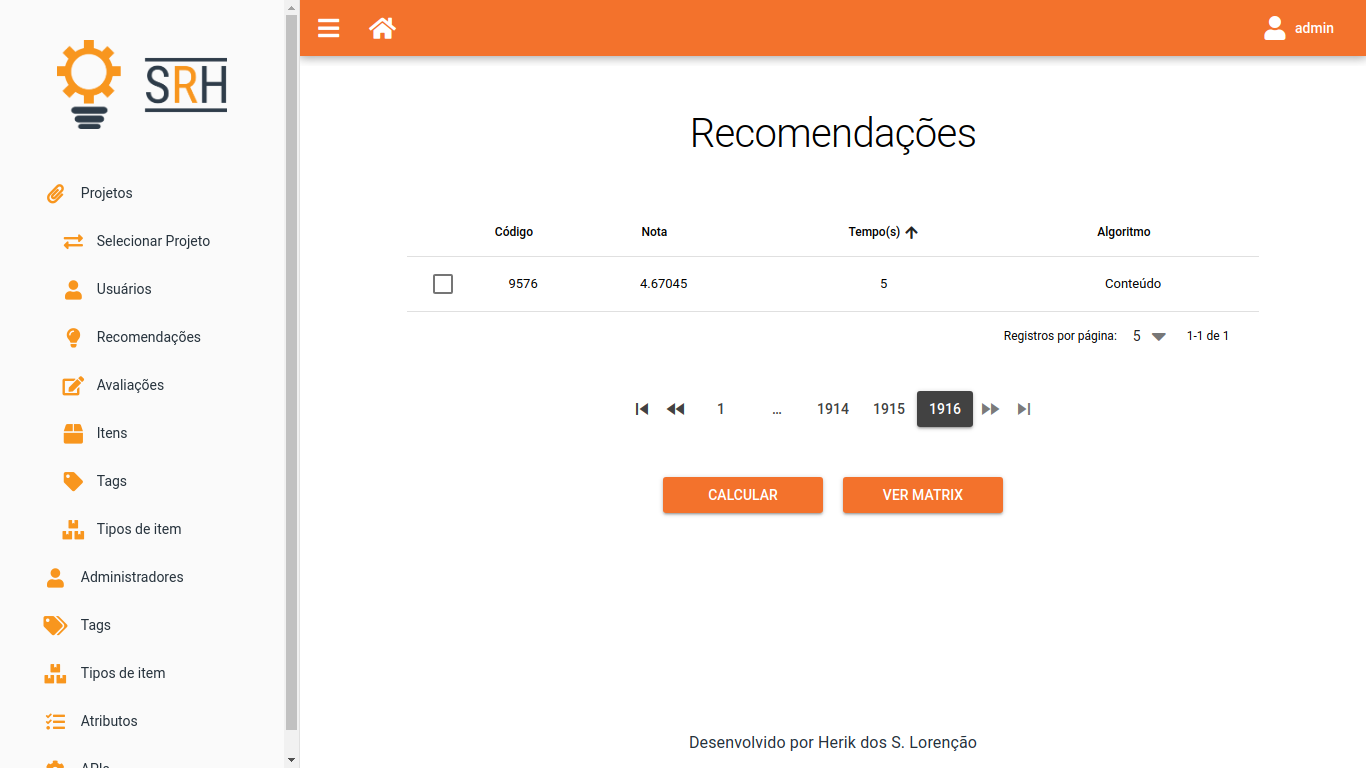
\includegraphics[width=.9\linewidth]{imagens/adminRecomendacoes.png}
	\caption[Cliente Administrativo: Recomendações]{Cliente Administrativo: Recomendações}
    \label{fig:clienteAdminRecomendacoes}
\end{figure}

\begin{figure}[H]
	\centering
	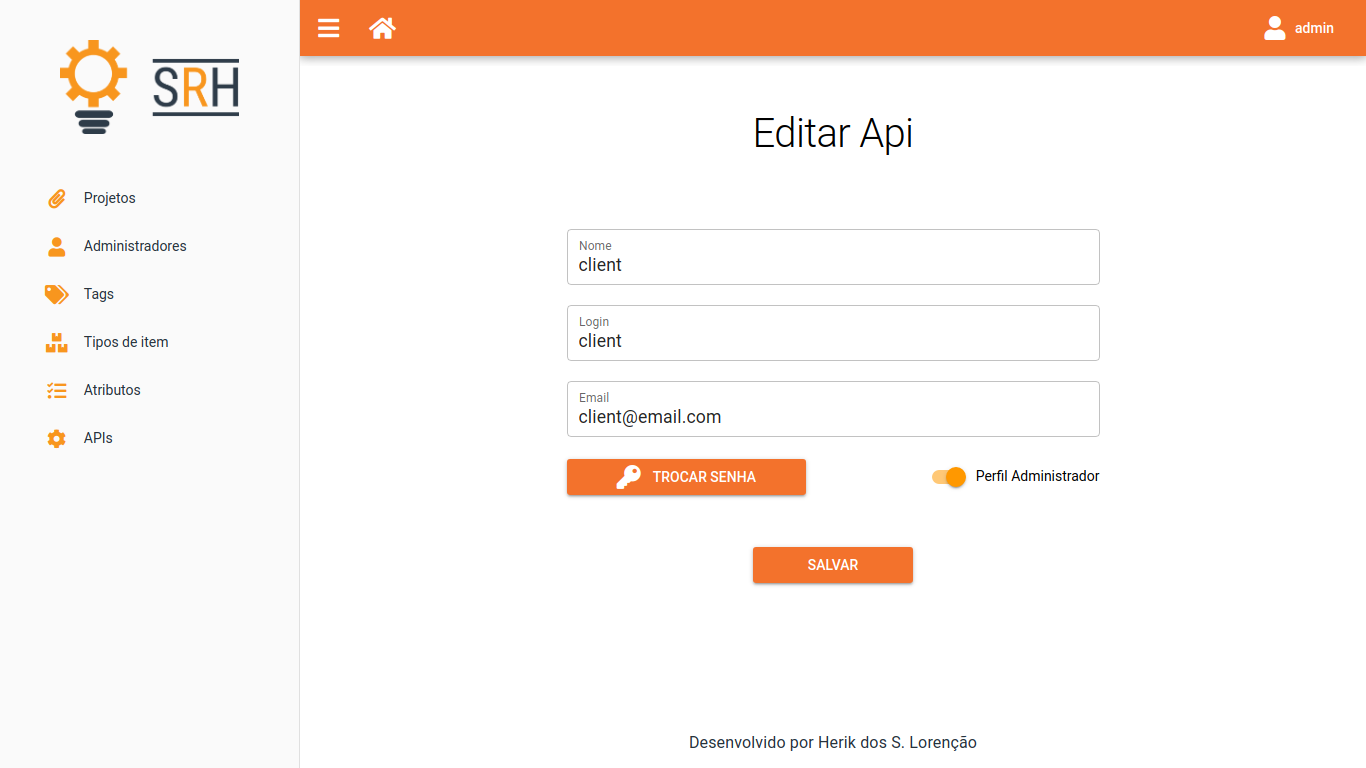
\includegraphics[width=.9\linewidth]{imagens/adminApi.png}
	\caption[Cliente Administrativo - Login]{Cliente Administrativo: Editar Usuário de API}
    \label{fig:clienteAdminUsuarioAPI}
\end{figure}

\subsection{Cliente de Recomendação}

Para que os avaliadores possam avaliar os itens em seus respectivos projetos foi desenvolvido uma aplicação cliente de recomendação, que permite o cadastro e acesso de um avaliador a um determinado projeto. Nas figuras \ref{fig:clienteLogin}, \ref{fig:clienteInicio}, \ref{fig:clienteAvaliacao}, \ref{fig:clienteAvaliacaoFinalizar} e \ref{fig:clienteEditarPerfil} pode-se visualizar algumas telas do sistema.

\begin{figure}[H]
	\centering
	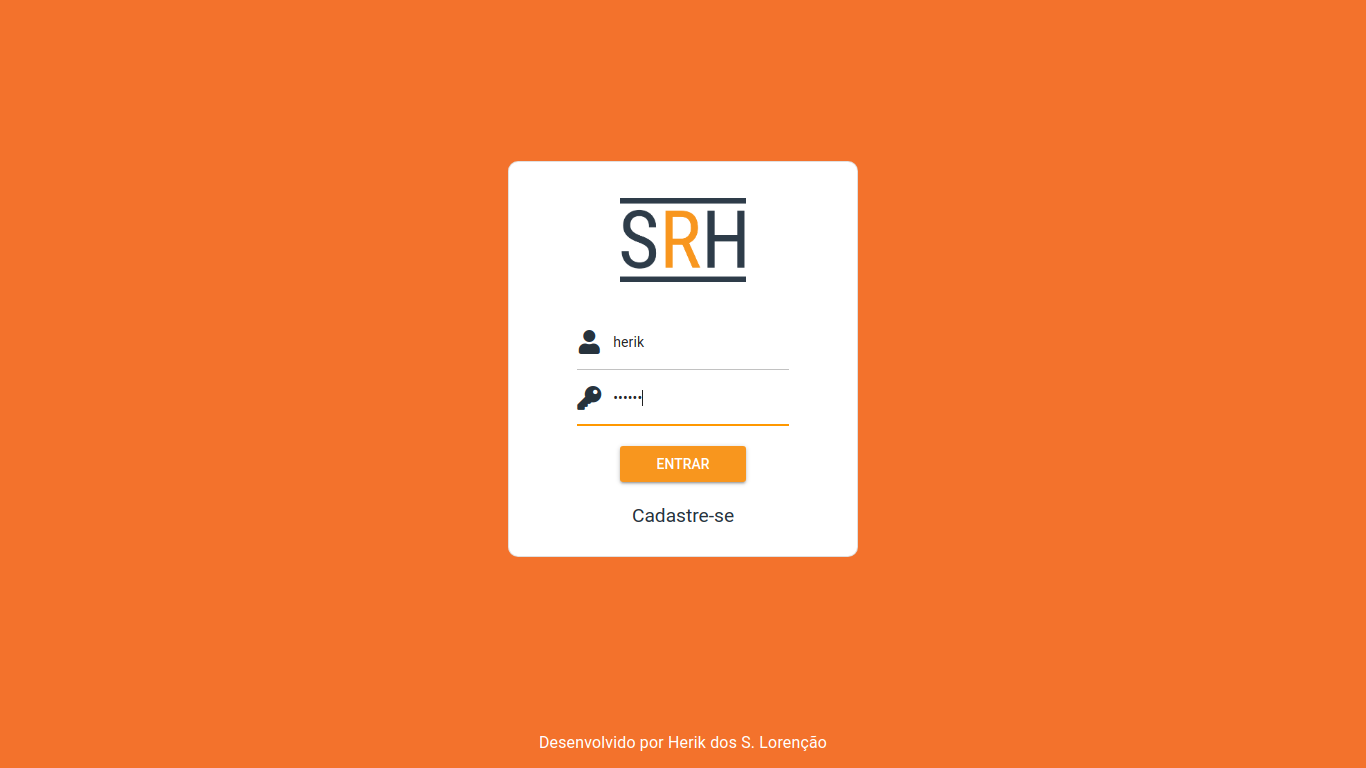
\includegraphics[width=.9\linewidth]{imagens/clientLogin.png}
	\caption[Cliente de Recomendação: Login]{Cliente de Recomendação: Login}
    \label{fig:clienteLogin}
\end{figure}

\begin{figure}[H]
	\centering
	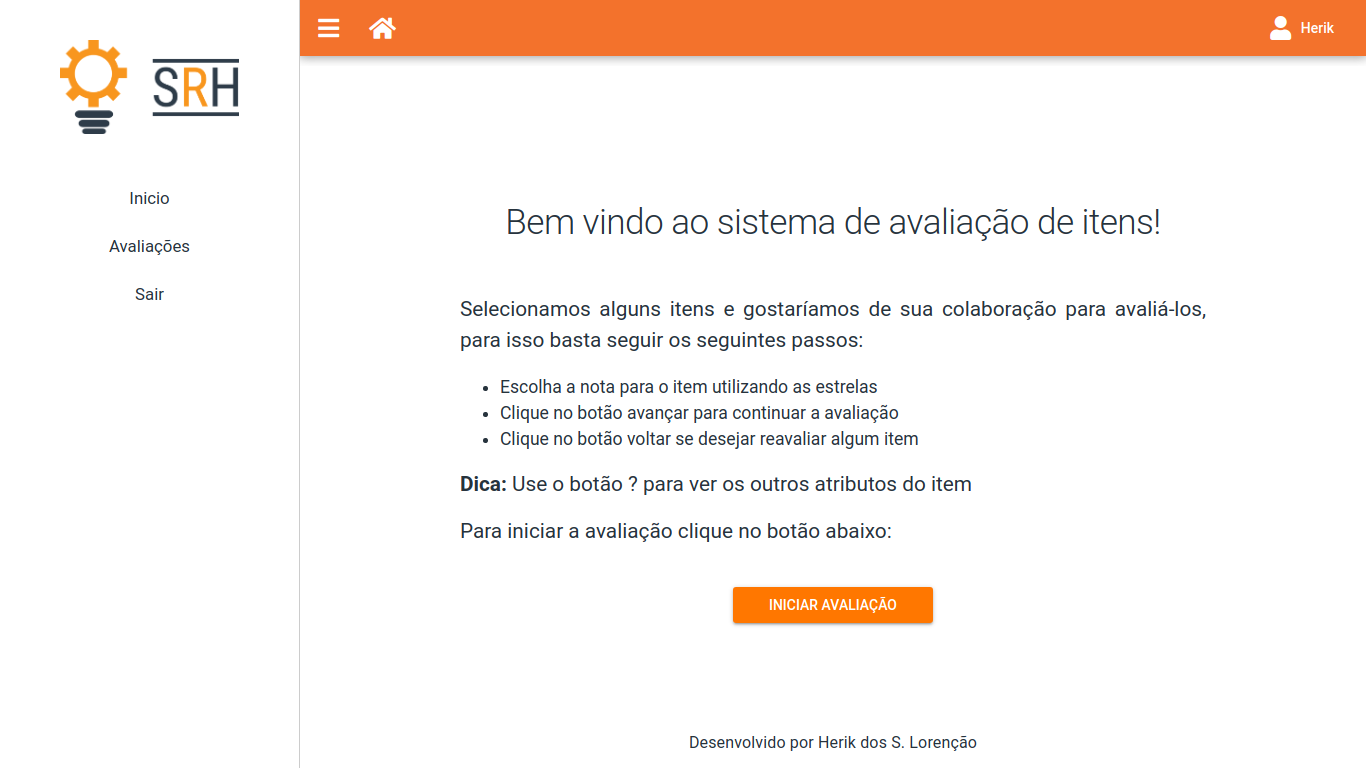
\includegraphics[width=.9\linewidth]{imagens/clientInicio.png}
	\caption[Cliente de Recomendação: Inicio]{Cliente de Recomendação: Inicio}
    \label{fig:clienteInicio}
\end{figure}

\begin{figure}[H]
	\centering
	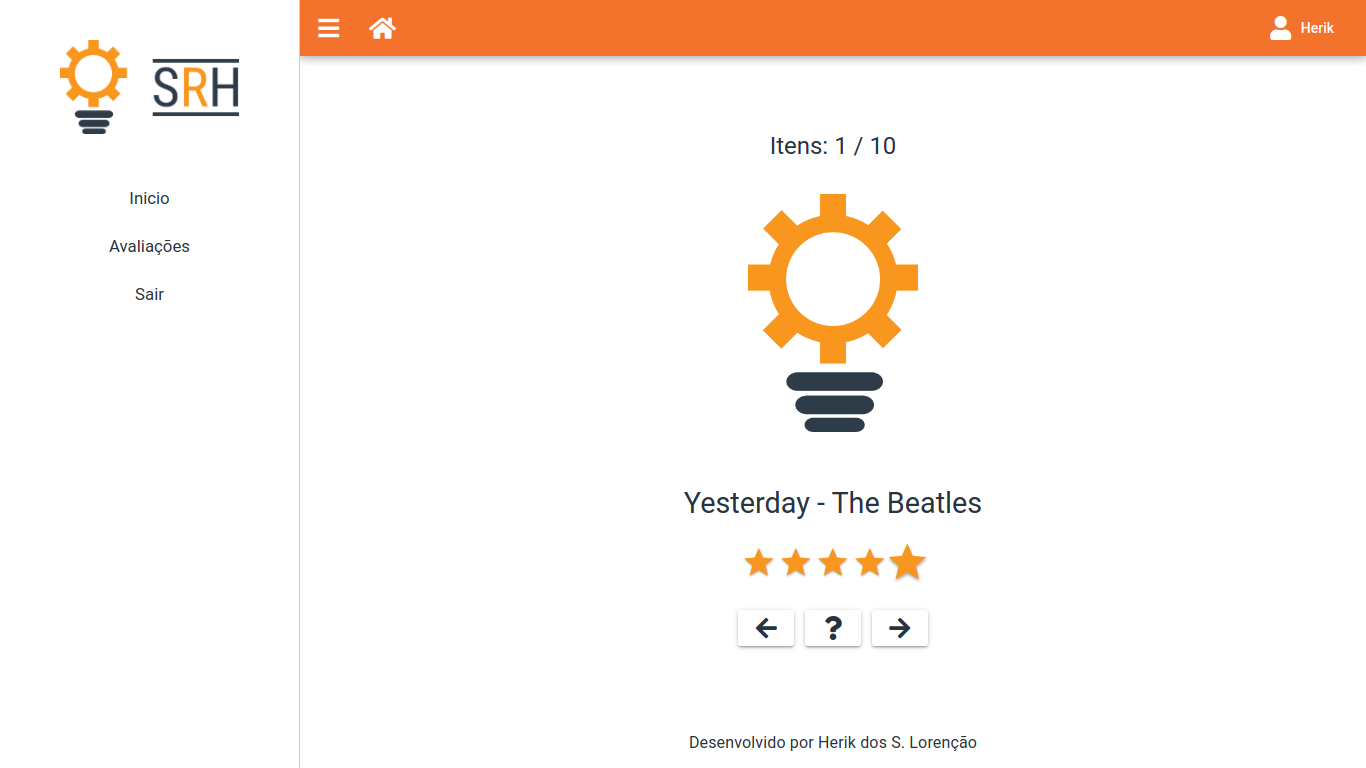
\includegraphics[width=.9\linewidth]{imagens/clientAvaliacao.png}
	\caption[Cliente de Recomendação: Avaliação]{Cliente de Recomendação: Avaliação}
    \label{fig:clienteAvaliacao}
\end{figure}

\begin{figure}[H]
	\centering
	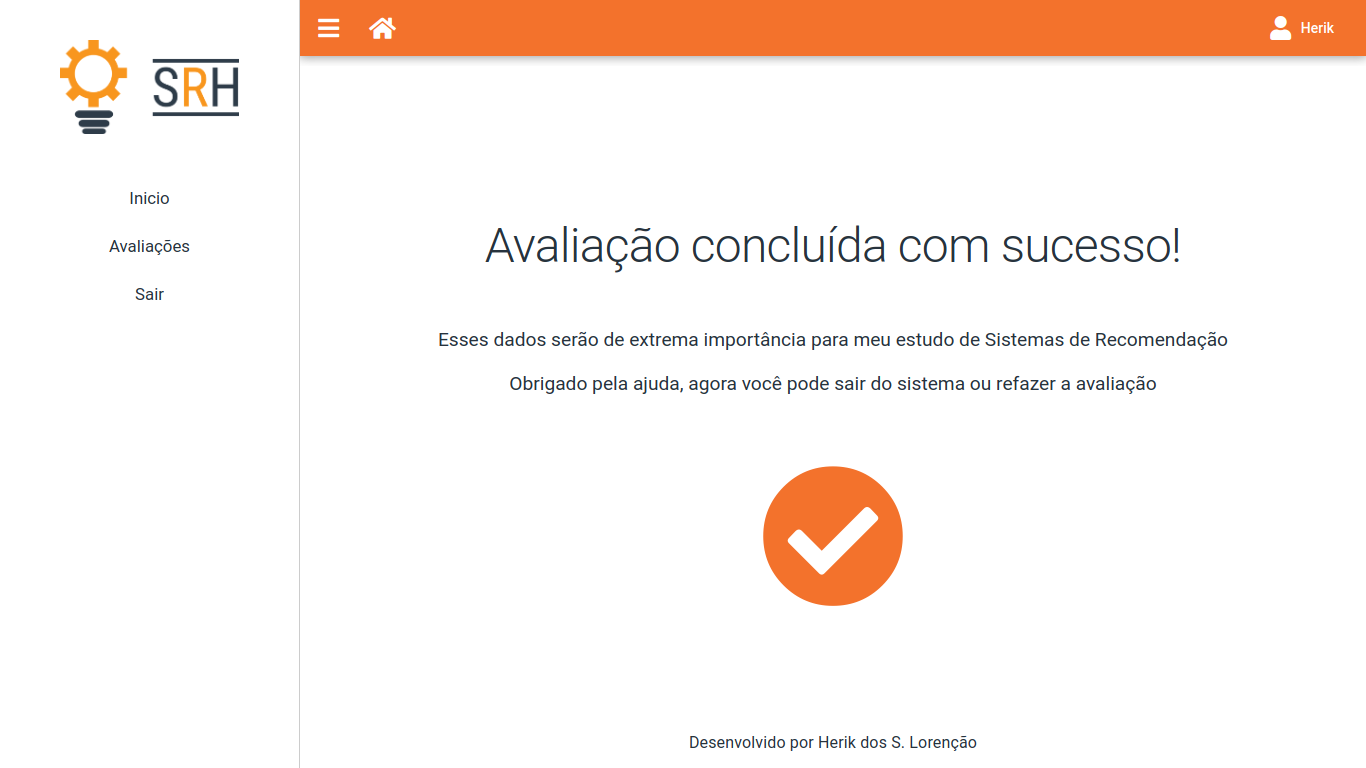
\includegraphics[width=.9\linewidth]{imagens/clientFinalizar.png}
	\caption[Cliente de Recomendação: Finalizar Avaliação]{Cliente de Recomendação: Finalizar Avaliação}
    \label{fig:clienteAvaliacaoFinalizar}
\end{figure}

\begin{figure}[H]
	\centering
	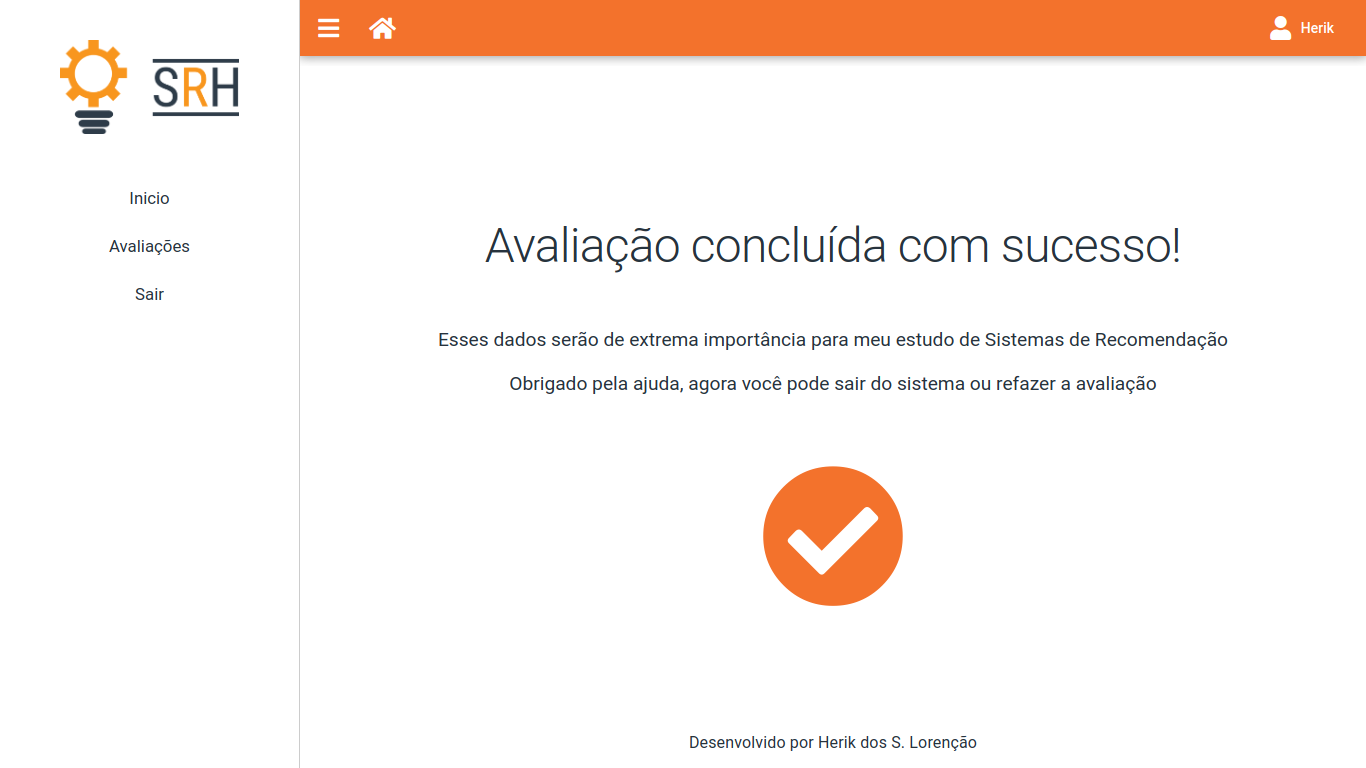
\includegraphics[width=.9\linewidth]{imagens/clientFinalizar.png}
	\caption[Cliente de Recomendação: Editar Perfil]{Cliente de Recomendação: Editar Perfil}
    \label{fig:clienteEditarPerfil}
\end{figure}

\section{Estudo de Caso: Educacional}

\subsection{Contexto}

O intuito deste estudo de caso foi recomendar exercícios aos alunos que pudessem auxiliar significativamente com seu aprendizado no conteúdo estudado.

Para desenvolvendo do estudo de caso, foi selecionada uma turma do curso técnico de Informática Integrado ao Ensino Médio do IFES - Campus Cachoeiro de Itapemirim. O objetivo era o de realizar perguntas relacionadas ao tema de estruturas de controle, na disciplina de Programação I.

Desse modo, o questionário foi aplicado na turma sendo pedido que todos os alunos respondessem todas as perguntas. Para avaliar a assertividade do sistema de recomendação, foram retiradas, de forma aleatória, um conjunto de 0 à 4 respostas de cada aluno, tendo como objetivo criar um ambiente para recomendação onde fosse possível avaliar a taxa de acerto das notas recomendadas.

Na tabela \ref{table:resultadosEstudoCasoEdu} é possível visualizar os dados acerca da pesquisa realizada:

\begin{table}[H]
\centering
\begin{tabular}{|c|c|}
\hline
\textbf{Itens}          & \textbf{Quantidade} \\ \hline
Número de alunos        & 29                  \\ \hline
Número de perguntas     & 9                   \\ \hline
Número de avaliações    & 214                 \\ \hline
Número de tags          & 9                   \\ \hline
Número de recomendações & 47                  \\ \hline
\end{tabular}
\label{table:resultadosEstudoCasoEdu} 
\end{table}

\subsection{Análise Descritiva}

Utilizando-se da estatística descritiva, pode-se avaliar a porcentagem de recomendações que foram aceitas pelos usuários do sistema, verificando, desse modo, sua taxa de acerto. Na figura \ref{fig:analiseDescritiva}, é possível avaliar os resultados obtidos nas recomendações como também as notas avaliadas pelos alunos para cada pergunta. A partir desses dados é possível realizar o processo de estatística descritiva.

\begin{figure}[H]
	\centering
	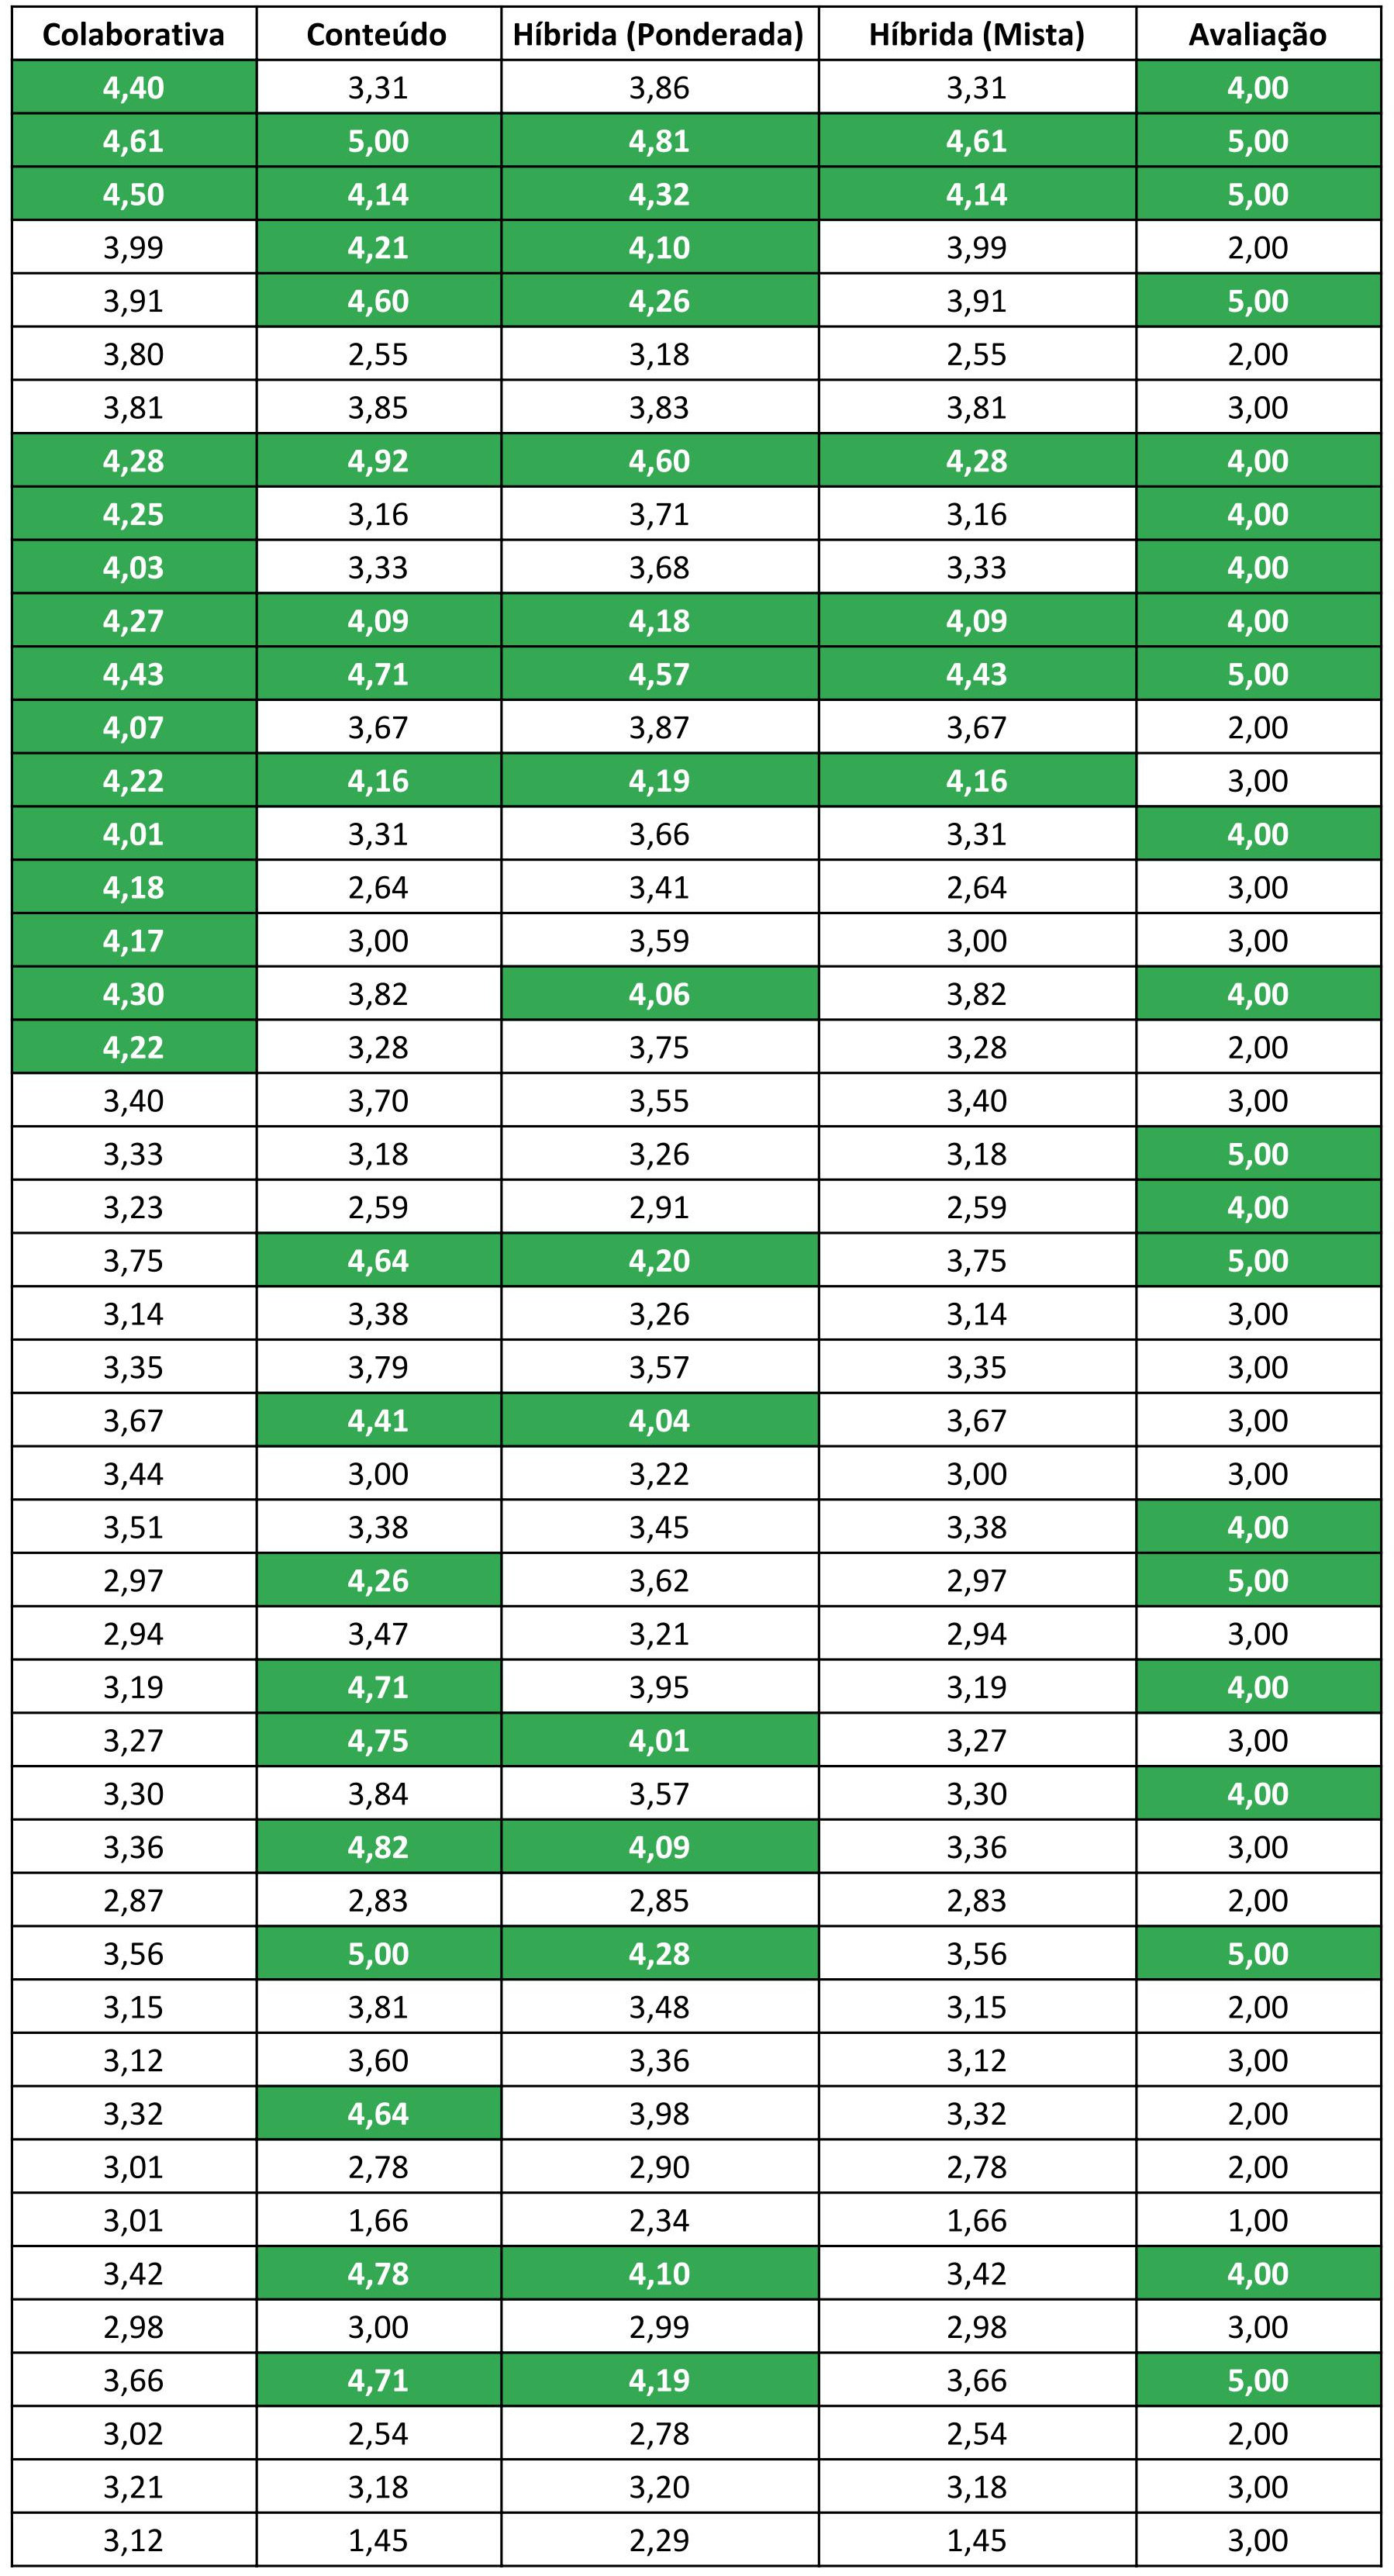
\includegraphics[width=0.8\linewidth]{imagens/estatisticaDescritiva.jpg}
	\caption[Estatística Descritiva]{Estatística Descritiva}
    \label{fig:analiseDescritiva}
\end{figure}

Avaliando as células marcadas na cor verde na figura \ref{fig:analiseDescritiva}, que representam os itens recomendados (notas maiores que o ponto de corte, definido como 4), é possível visualizar a quantidade de acertos e erros das abordagens de recomendação em relação as notas avaliadas pelos usuários. Esses dados são apresentados na figura \ref{fig:analiseDescritivaTaxas}:

\begin{figure}[H]
	\centering
	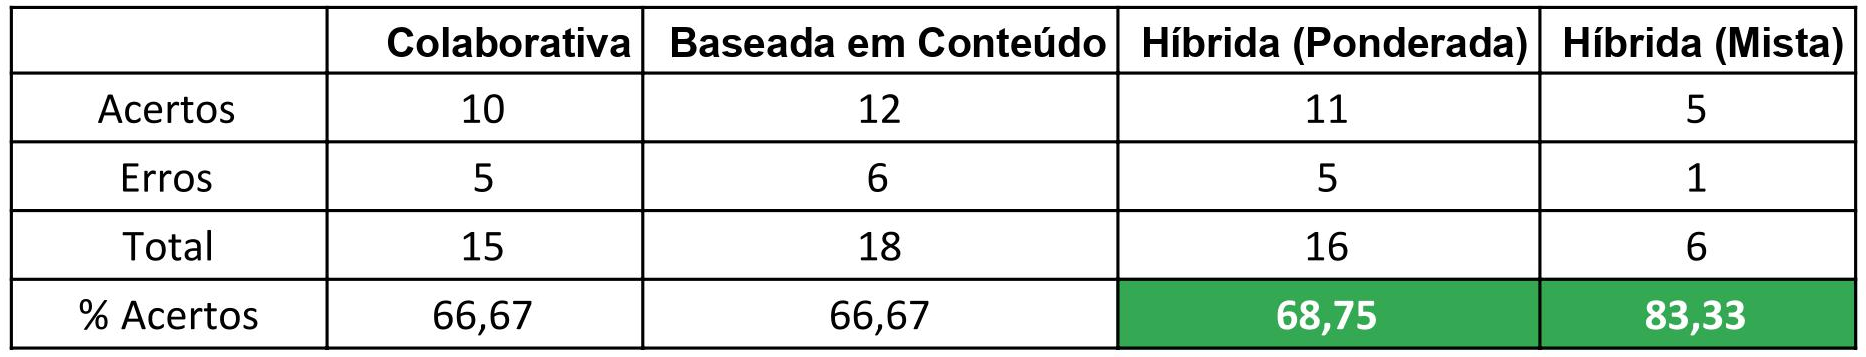
\includegraphics[width=.9\linewidth]{imagens/analiseDescritivaTaxas.jpg}
	\caption[Taxas da Estatística Descritiva]{Taxas da Estatística Descritiva}
    \label{fig:analiseDescritivaTaxas}
\end{figure}

A partir dos dados disponíveis na figura \ref{fig:analiseDescritivaTaxas}, conclui-se que as abordagens híbridas (marcadas com a cor verde) obtiveram um resultado superior as abordagens colaborativas e baseada em conteúdo no estudo analisado. Vale ressaltar o resultado obtido na abordagem híbrida mista, que apresentou um resultado 16,66\% superior as abordagens não híbridas.

\subsection{Testes em T}

Como forma de avaliar os resultados sobre outra perspectiva e metodologia, foram realizados os testes em T que representam outra forma de análise estatística. Nesse tipo de análise, é buscado verificar a diferença entre as médias das recomendações e as avaliações dos estudantes, buscando a menor divergência possível entre os resultados.

\begin{figure}[H]
	\centering
	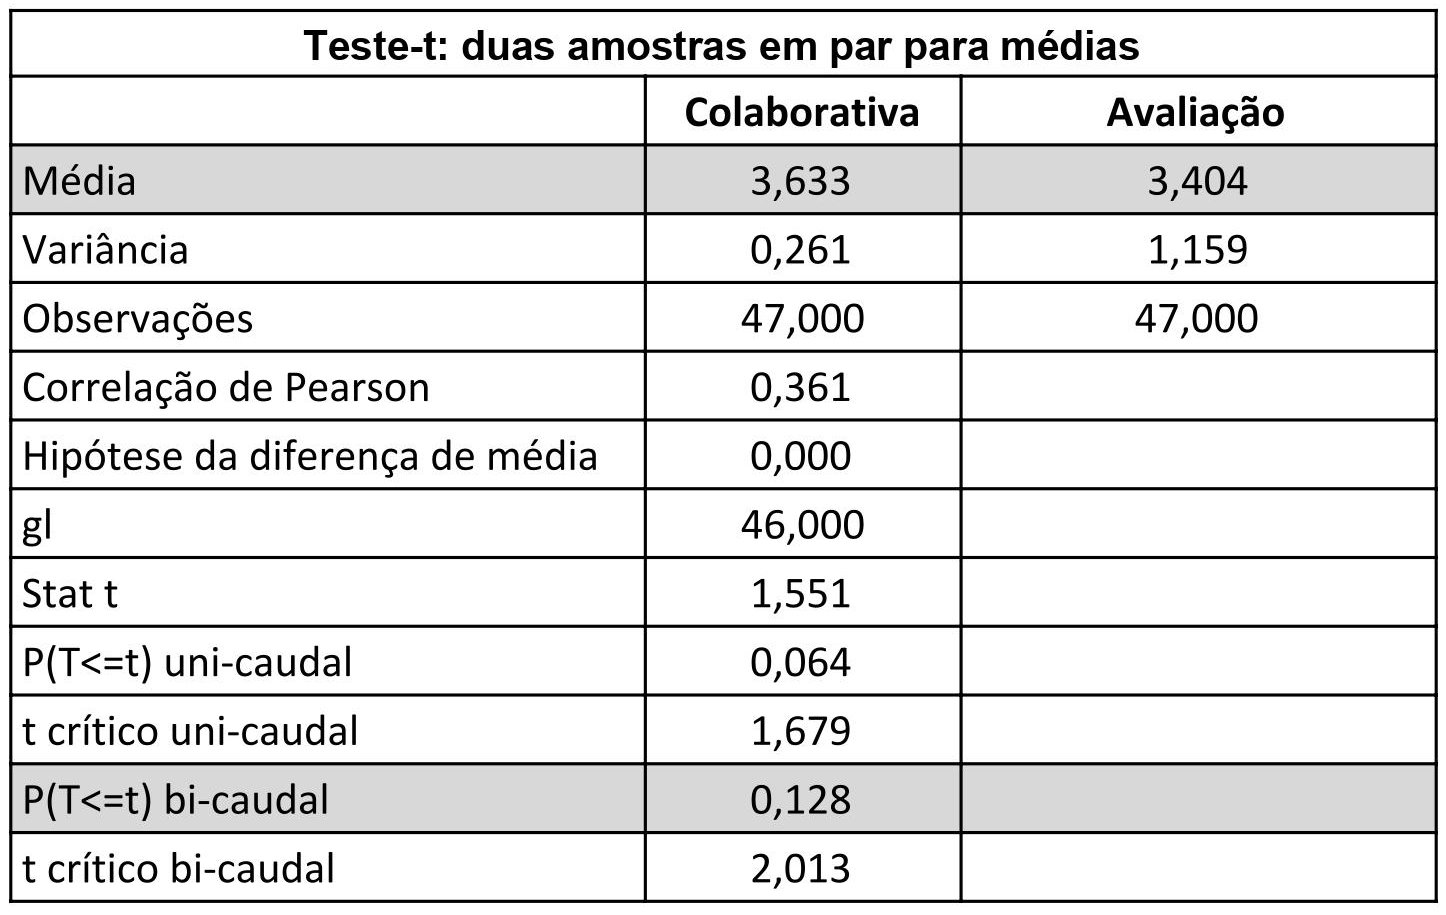
\includegraphics[width=.7\linewidth]{imagens/testeTColaborativa.jpg}
	\caption[Teste T: Filtragem Colaborativa]{Teste T: Filtragem Colaborativa}
    \label{fig:testeTColaborativa}
\end{figure}

A partir dos resultados obtidos na figura \ref{fig:testeTColaborativa}, pode-se observar que o valor de \textbf{P(t<=t) bi-caudal} é superior a \textbf{0,05}. Isso significa que as recomendações para filtragem colaborativa foram boas, uma vez que apresentam similaridade com as avaliações dos usuários.

\begin{figure}[H]
	\centering
	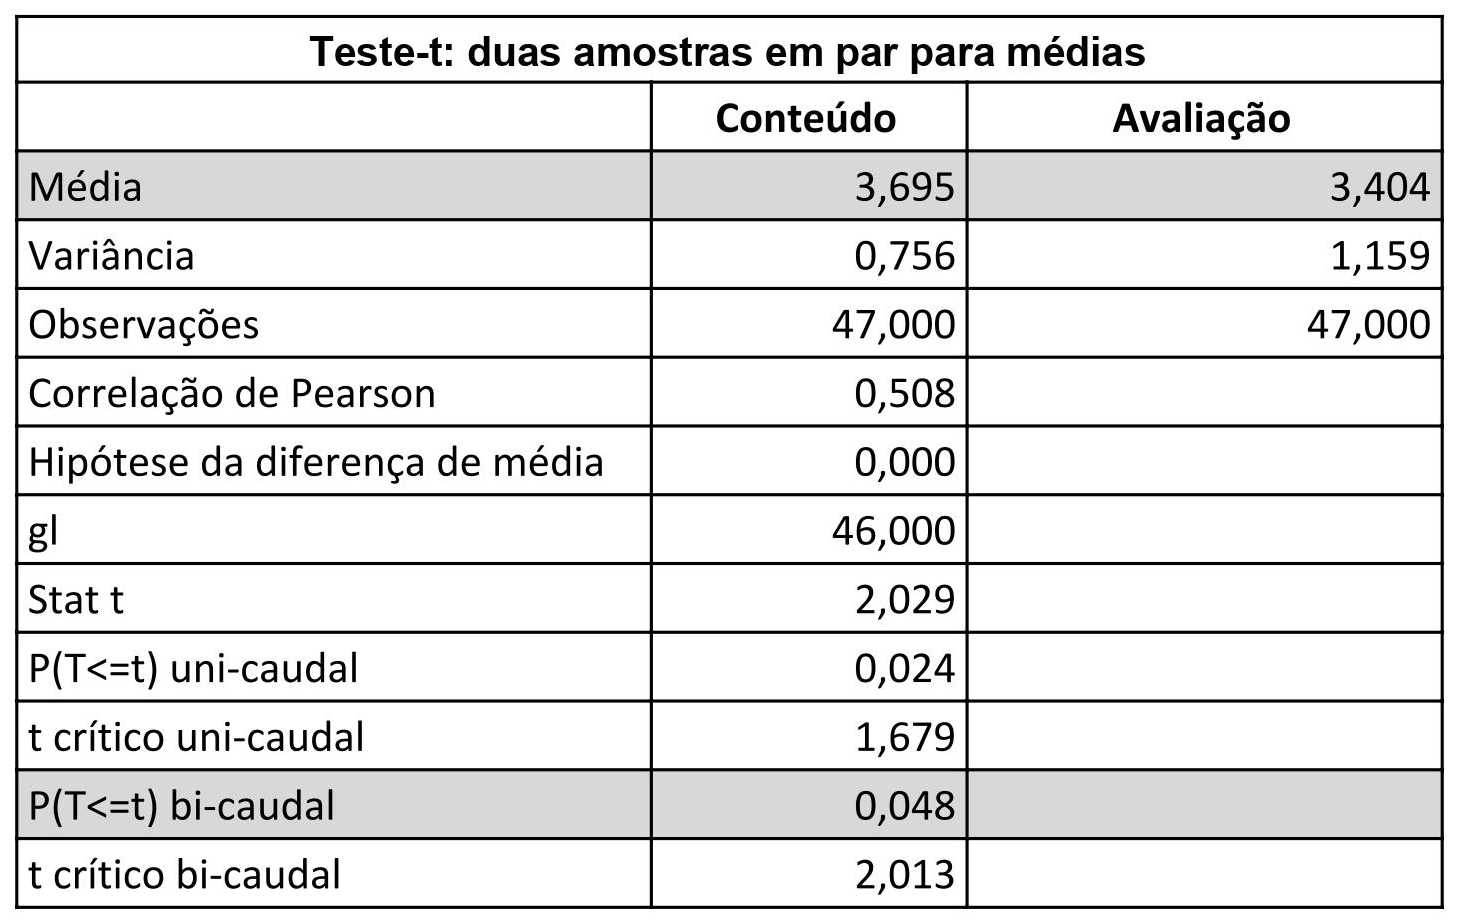
\includegraphics[width=.7\linewidth]{imagens/testeTConteudo.jpg}
	\caption[Teste T: Filtragem Baseada em Conteúdo]{Teste T: Filtragem Baseada em Conteúdo}
    \label{fig:testeTConteudo}
\end{figure}

Os resultados para filtragem baseada em conteúdo, apresentados na figura \ref{fig:testeTConteudo} demonstram um valor para \textbf{P(t<=t) bi-caudal} inferior a \textbf{0,05}. Com isso, é observado que existem uma divergência entre os resultados das recomendações baseadas em conteúdo se comparado com as avaliações dos usuários.

\begin{figure}[H]
	\centering
	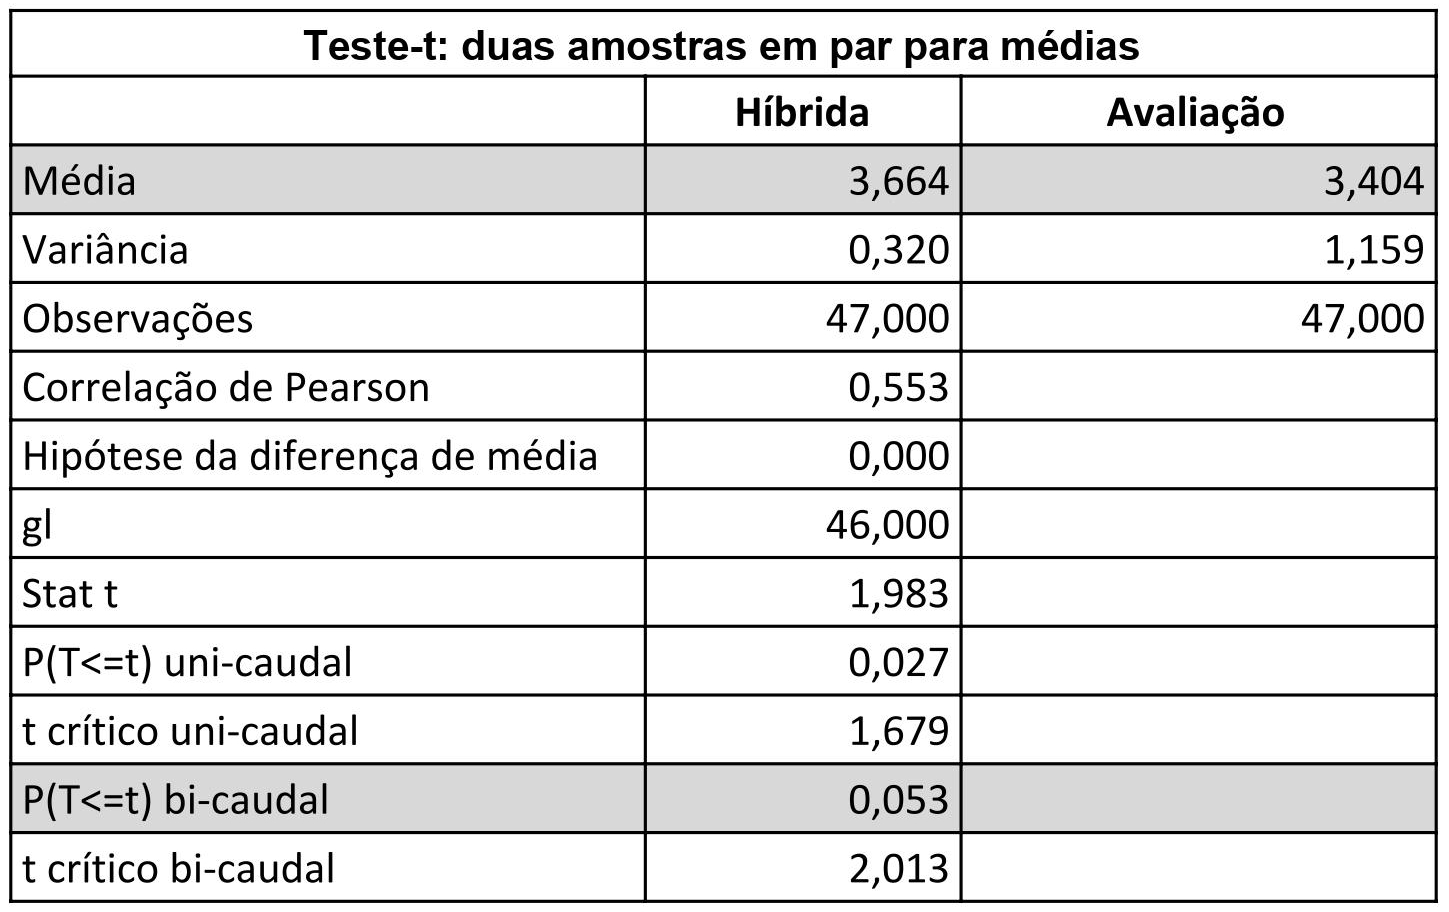
\includegraphics[width=.7\linewidth]{imagens/testeTPonderada.jpg}
	\caption[Teste T: Filtragem Híbrida Ponderada]{Filtragem Híbrida Ponderada}
    \label{fig:testeTPonderado}
\end{figure}

A partir das informações mostradas na figura \ref{fig:testeTPonderado}, é possível analisar que o valor \textbf{P(t<=t) bi-caudal} é superior a \textbf{0,05}. Isso demonstra que as recomendações geradas na filtragem híbrida ponderada apresentam similaridade com as avaliações dos usuários.

\begin{figure}[H]
	\centering
	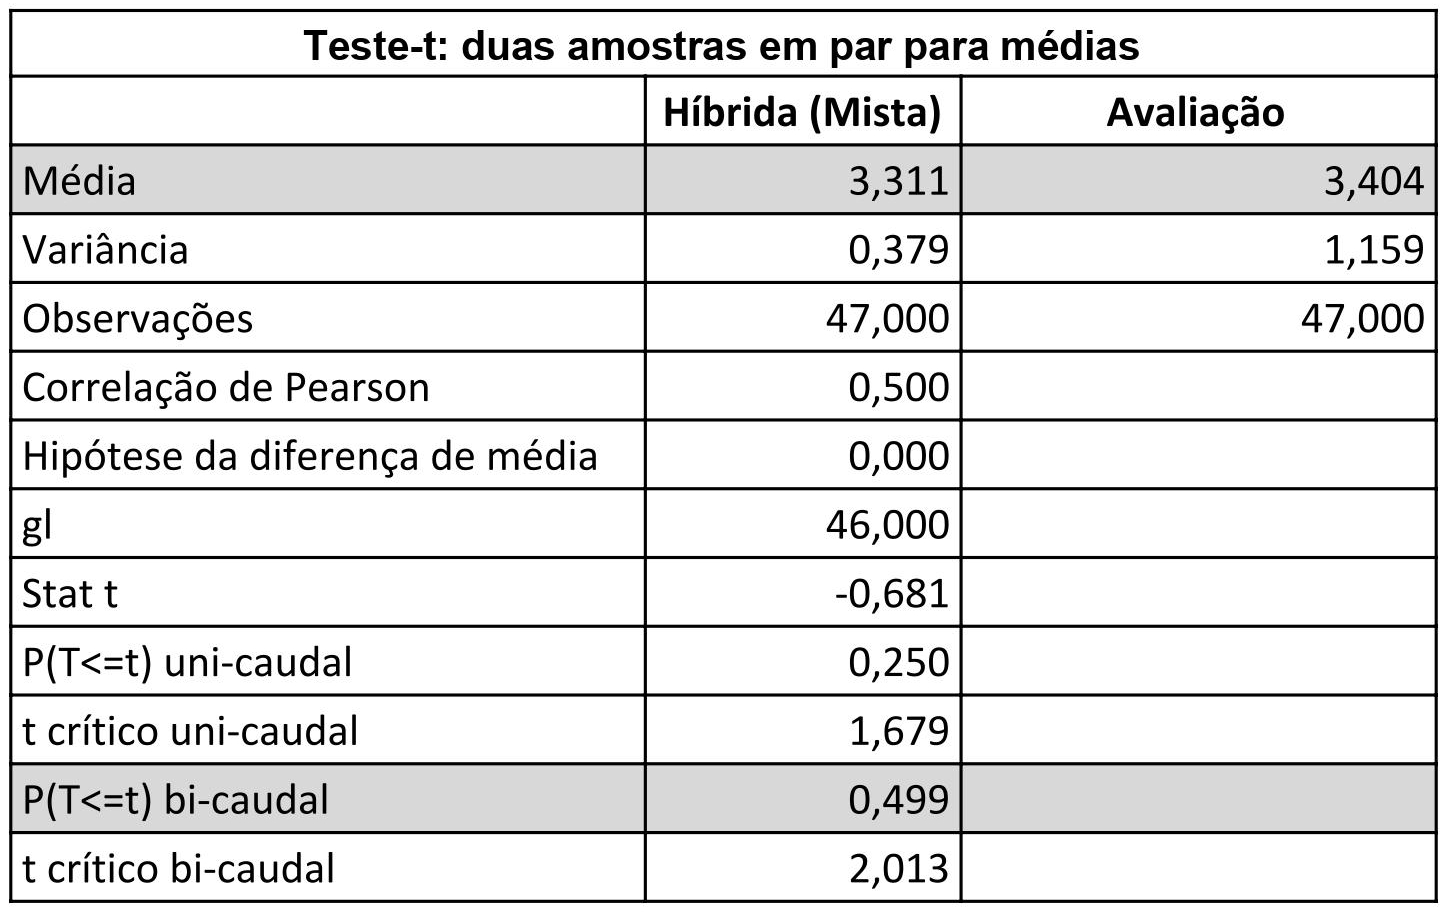
\includegraphics[width=.7\linewidth]{imagens/testeTMisto.jpg}
	\caption[Teste T: Filtragem Híbrida Mista]{Filtragem Híbrida Mista}
    \label{fig:testeTMisto}
\end{figure}

Os resultados da filtragem híbrida mista, apresentados na figura \ref{fig:testeTMisto} demonstram que o valor \textbf{P(t<=t) bi-caudal} é inferior a \textbf{0,05}. Desse modo, é possível observar que existem divergências entre os resultados apresentados pela filtragem híbrida mista e as avaliações dos usuários.

\section{Estudo de Caso: Recomendação de Músicas}

\subsection{Contexto}

No estudo de caso realizado foi avaliado o gosto musical de diversas pessoas acerca de 10 músicas previamente selecionadas, compondo um repertório bastante variado, permitindo a definição de diversas Tags para recomendação.

Para a elaboração desse estudo foi desenvolvida uma aplicação web contextualizada para o ambiente musical, como apresentado nas figuras \ref{fig:findmusicLogin}, \ref{fig:findmusicInicio} e \ref{fig:findmusicAvaliacao}. Essa aplicação foi disponibilizada e divulgada na internet, possibilitando o acesso das pessoas que tivessem interesse.

\begin{figure}[H]
	\centering
	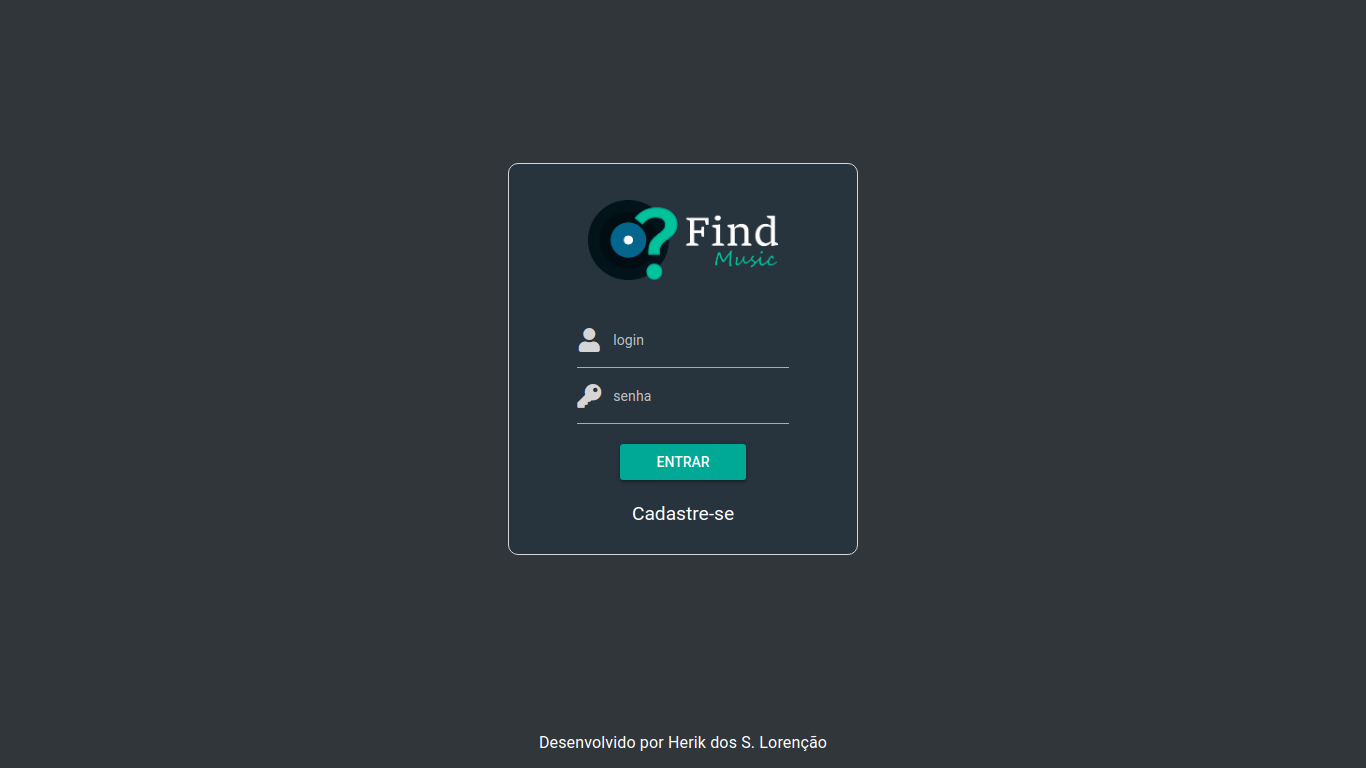
\includegraphics[width=.7\linewidth]{imagens/findmusicLogin.png}
	\caption[Aplicação cliente: Tela de Login]{Aplicação cliente: Tela de Login}
    \label{fig:findmusicLogin}
\end{figure}

\begin{figure}[H]
	\centering
	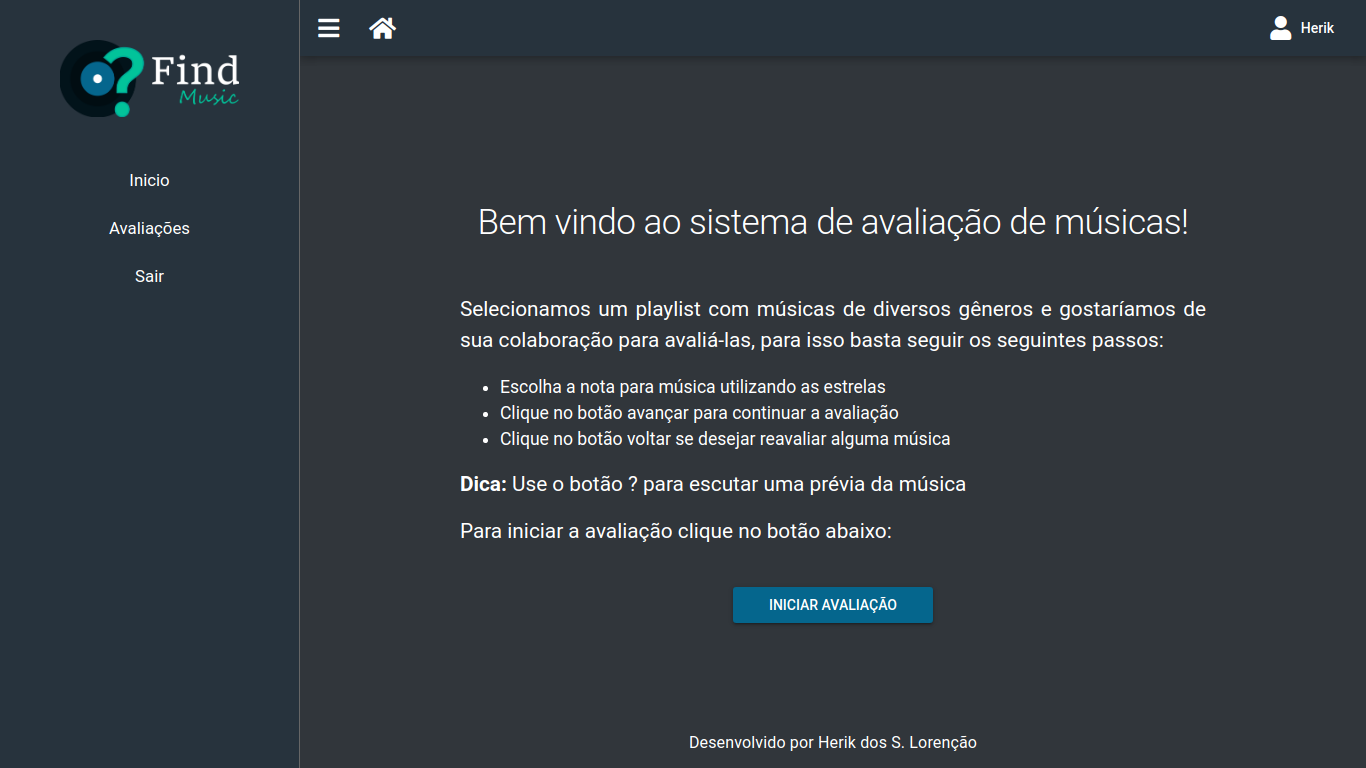
\includegraphics[width=.7\linewidth]{imagens/findmusicInicio.png}
	\caption[Aplicação cliente: Tela Inicial]{Aplicação cliente: Tela Inicial}
    \label{fig:findmusicInicio}
\end{figure}

\begin{figure}[H]
	\centering
	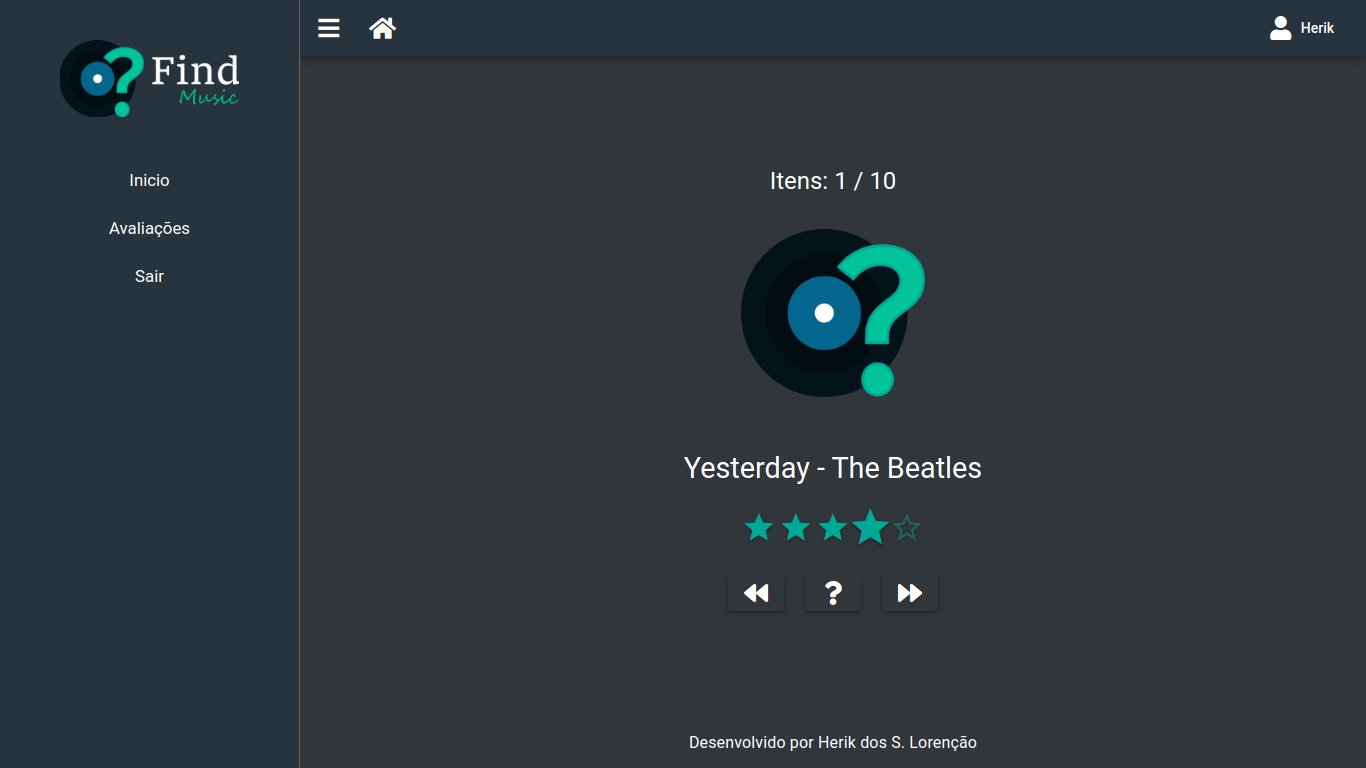
\includegraphics[width=.7\linewidth]{imagens/findmusicAvaliacao.png}
	\caption[Aplicação cliente: Avaliação]{Aplicação cliente: Avaliação}
    \label{fig:findmusicAvaliacao}
\end{figure}

A partir das avaliações recebidas foram selecionadas de forma e quantidade aleatório valores para serem retirados das avaliações de cada avaliador, com isso, foi possível realizar o processo de recomendação e comparar o resultado recomendado com o avaliado pelo usuário. Dese modo, foi possível obter os seguintes dados:

\begin{table}[H]
\centering
\begin{tabular}{|c|c|}
\hline
\textbf{Itens}          & \textbf{Quantidade} \\ \hline
Número de avaliadores   & 60                  \\ \hline
Número de músicas       & 10                  \\ \hline
Número de avaliações    & 600                 \\ \hline
Número de tags          & 6                   \\ \hline
Número de recomendações & 141                  \\ \hline
\end{tabular}
\label{table:resultadosEstudoCasoEdu} 
\end{table}

\subsection{Análise Descritiva}

Utilizando-se da análise descritiva foi possível definir a taxa de acerto do sistema sobre as recomendações que seriam aceitas pelos usuários. Nas figuras \ref{fig:findMusicEstatistica1}, \ref{fig:findMusicEstatistica2}, \ref{fig:findMusicEstatistica3} e \ref{fig:findMusicEstatistica4} pode ser observado a comparação entre as notas geradas pelas estratégias de recomendação e a nota real informada pelo usuário, o que possibilita a realização do processo de estatística descritiva.

\begin{figure}[H]
	\centering
	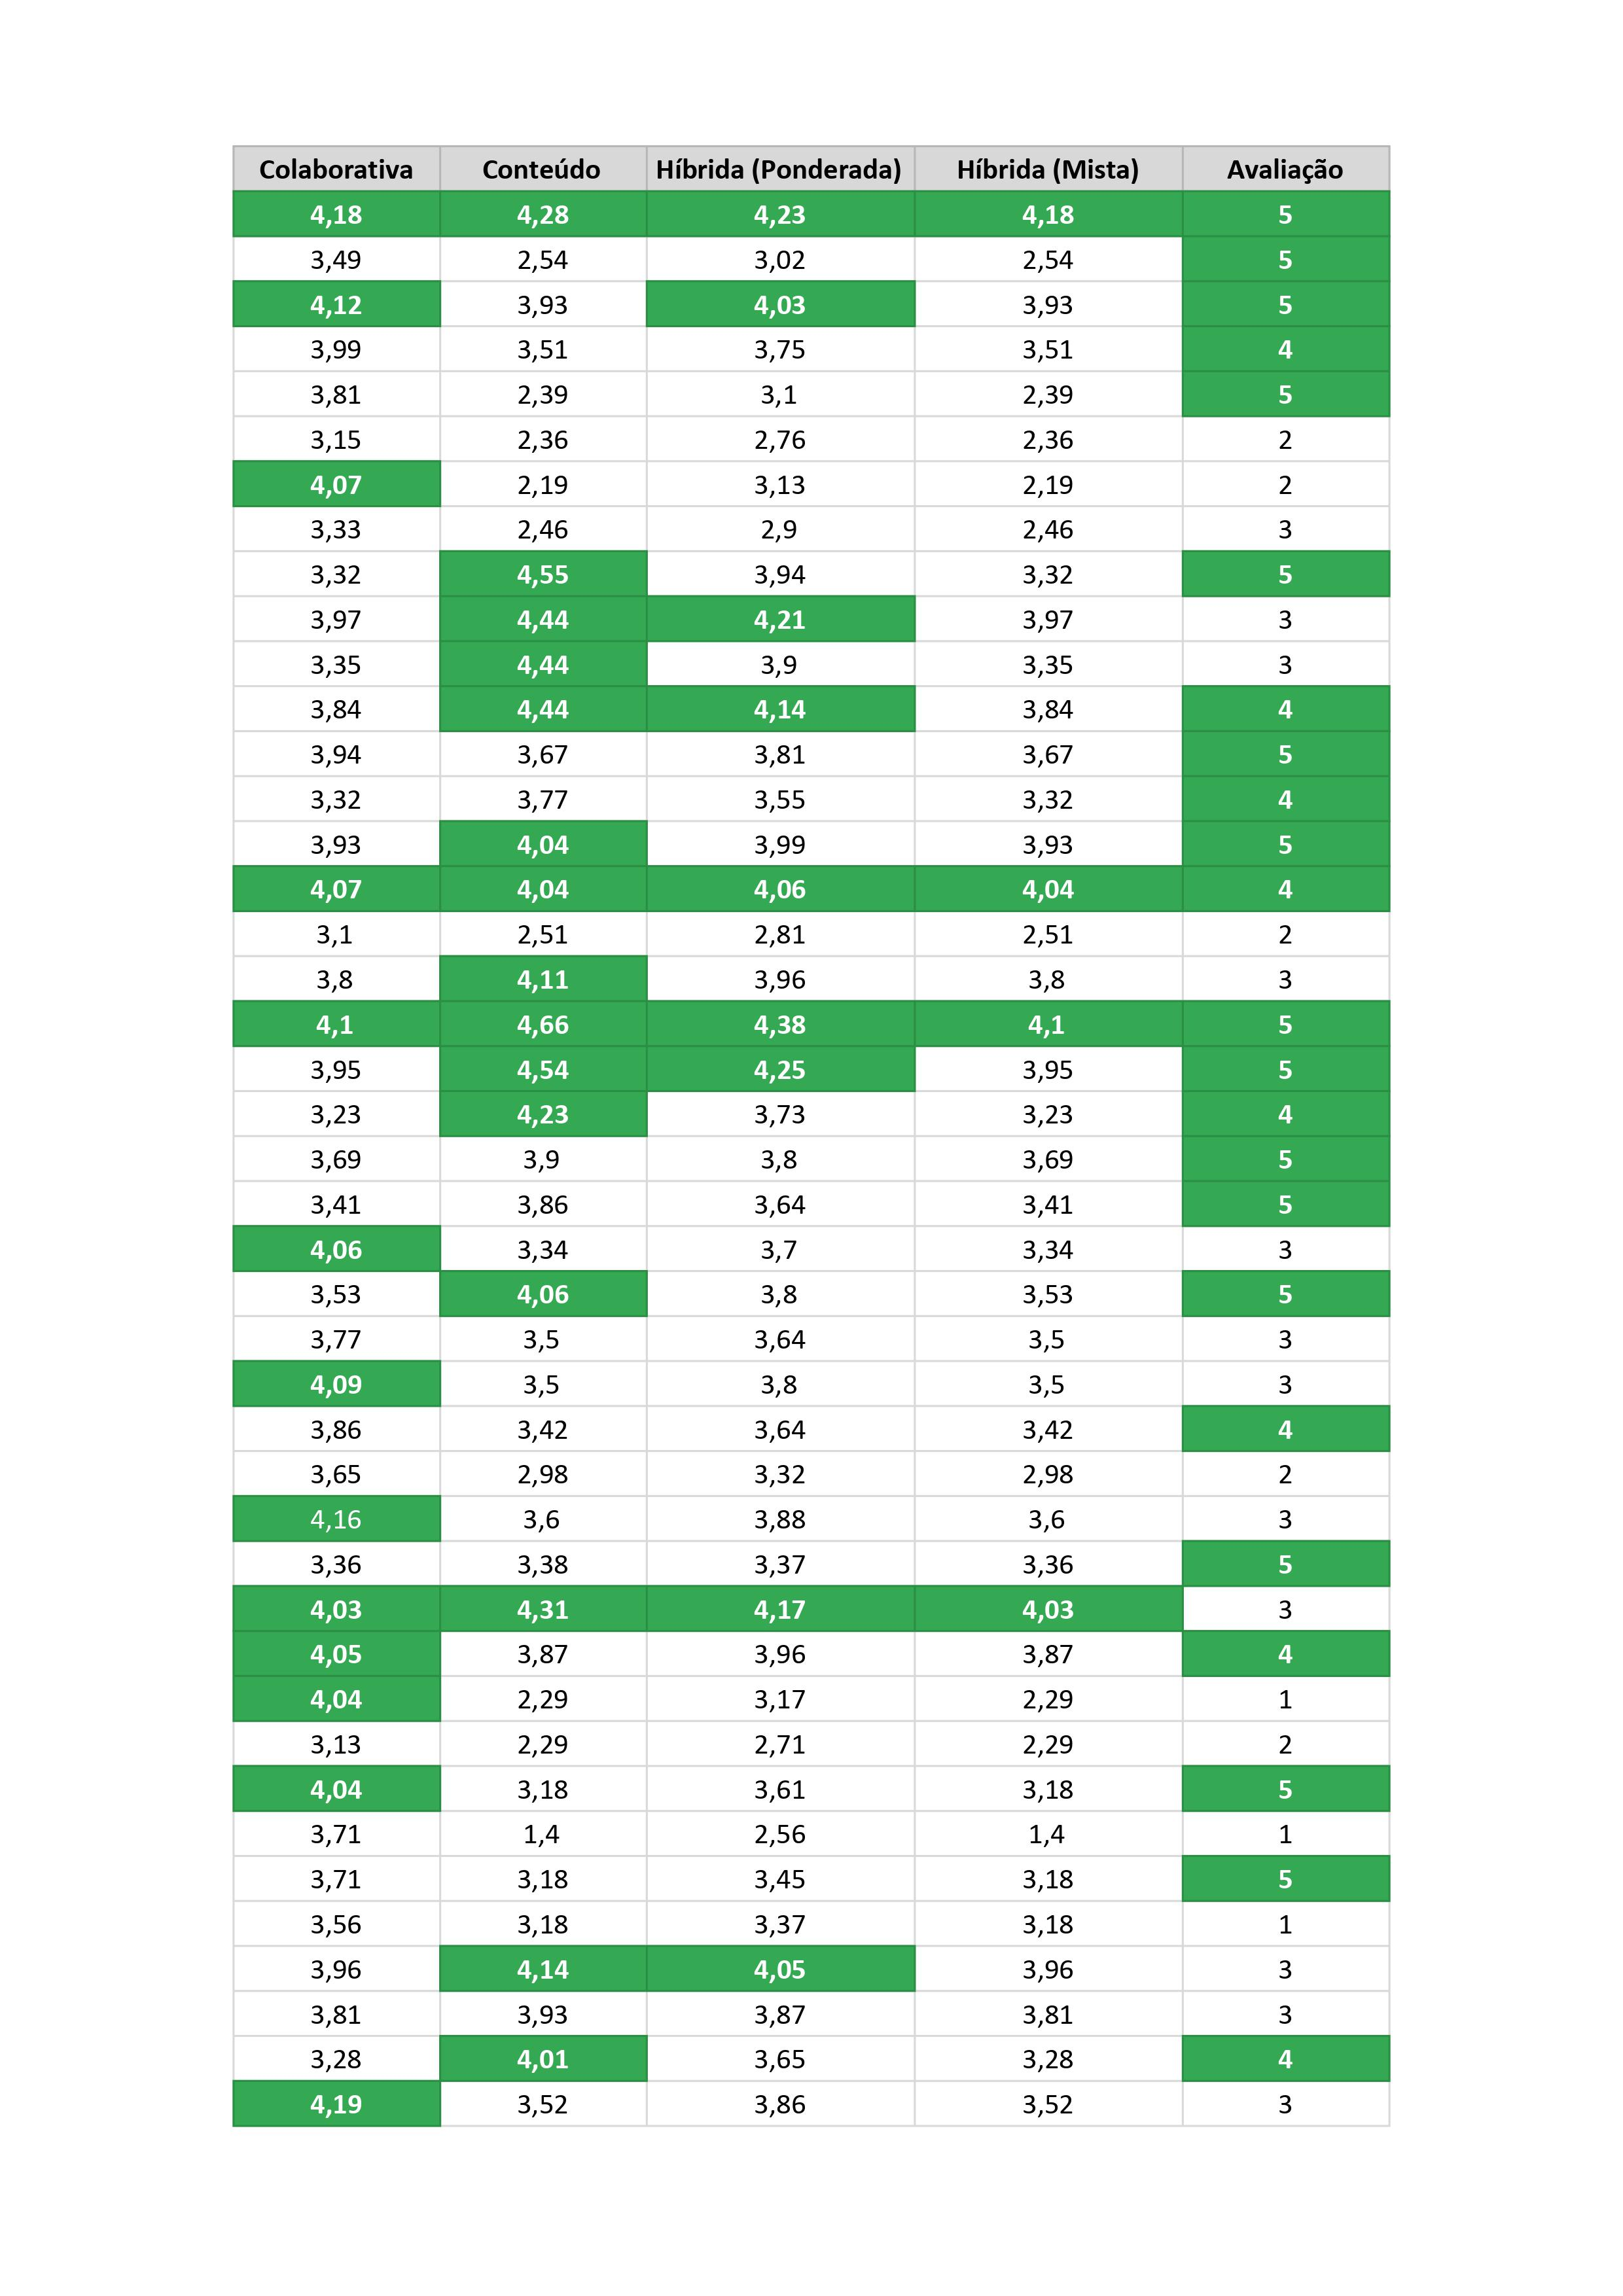
\includegraphics[width=1\linewidth]{imagens/findMusicResultados1.jpg}
	\caption[Estatística Descritiva: Parte 1]{Estatística Descritiva: Parte 1}
    \label{fig:findMusicEstatistica1}
\end{figure}

\begin{figure}[H]
	\centering
	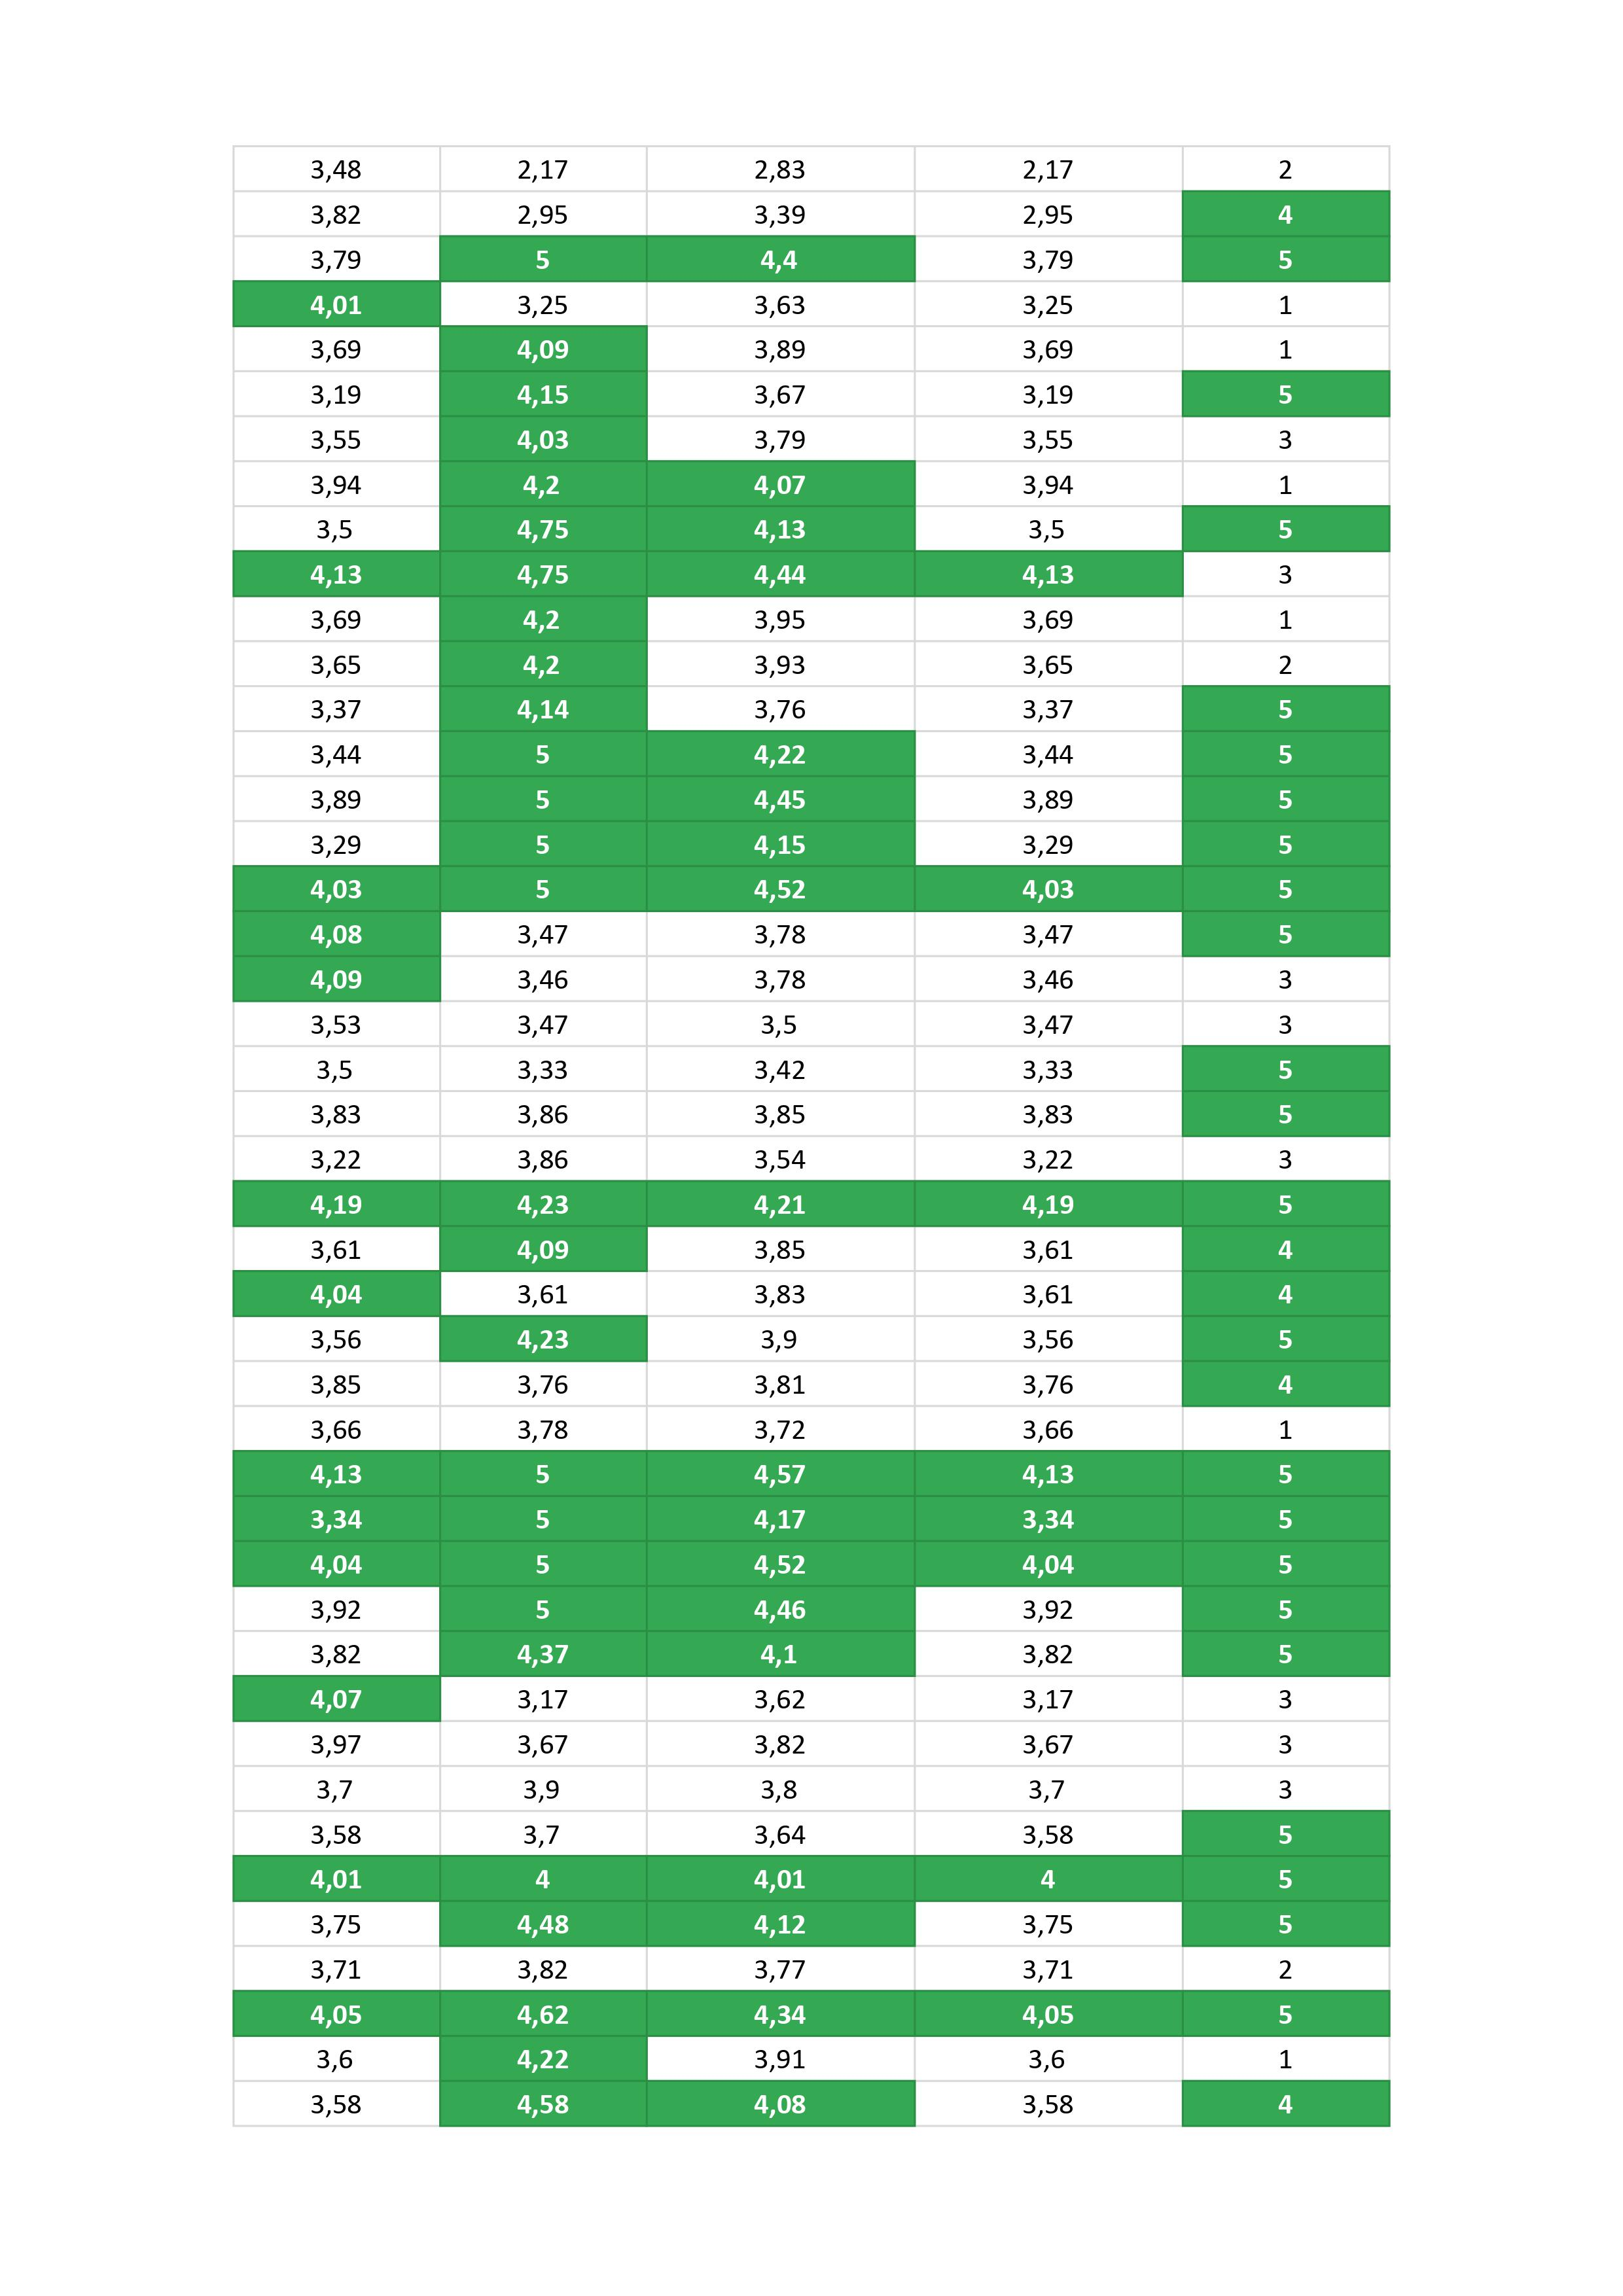
\includegraphics[width=1\linewidth]{imagens/findMusicResultados2.jpg}
	\caption[Estatística Descritiva: Parte 2]{Estatística Descritiva: Parte 2}
    \label{fig:findMusicEstatistica2}
\end{figure}

\begin{figure}[H]
	\centering
	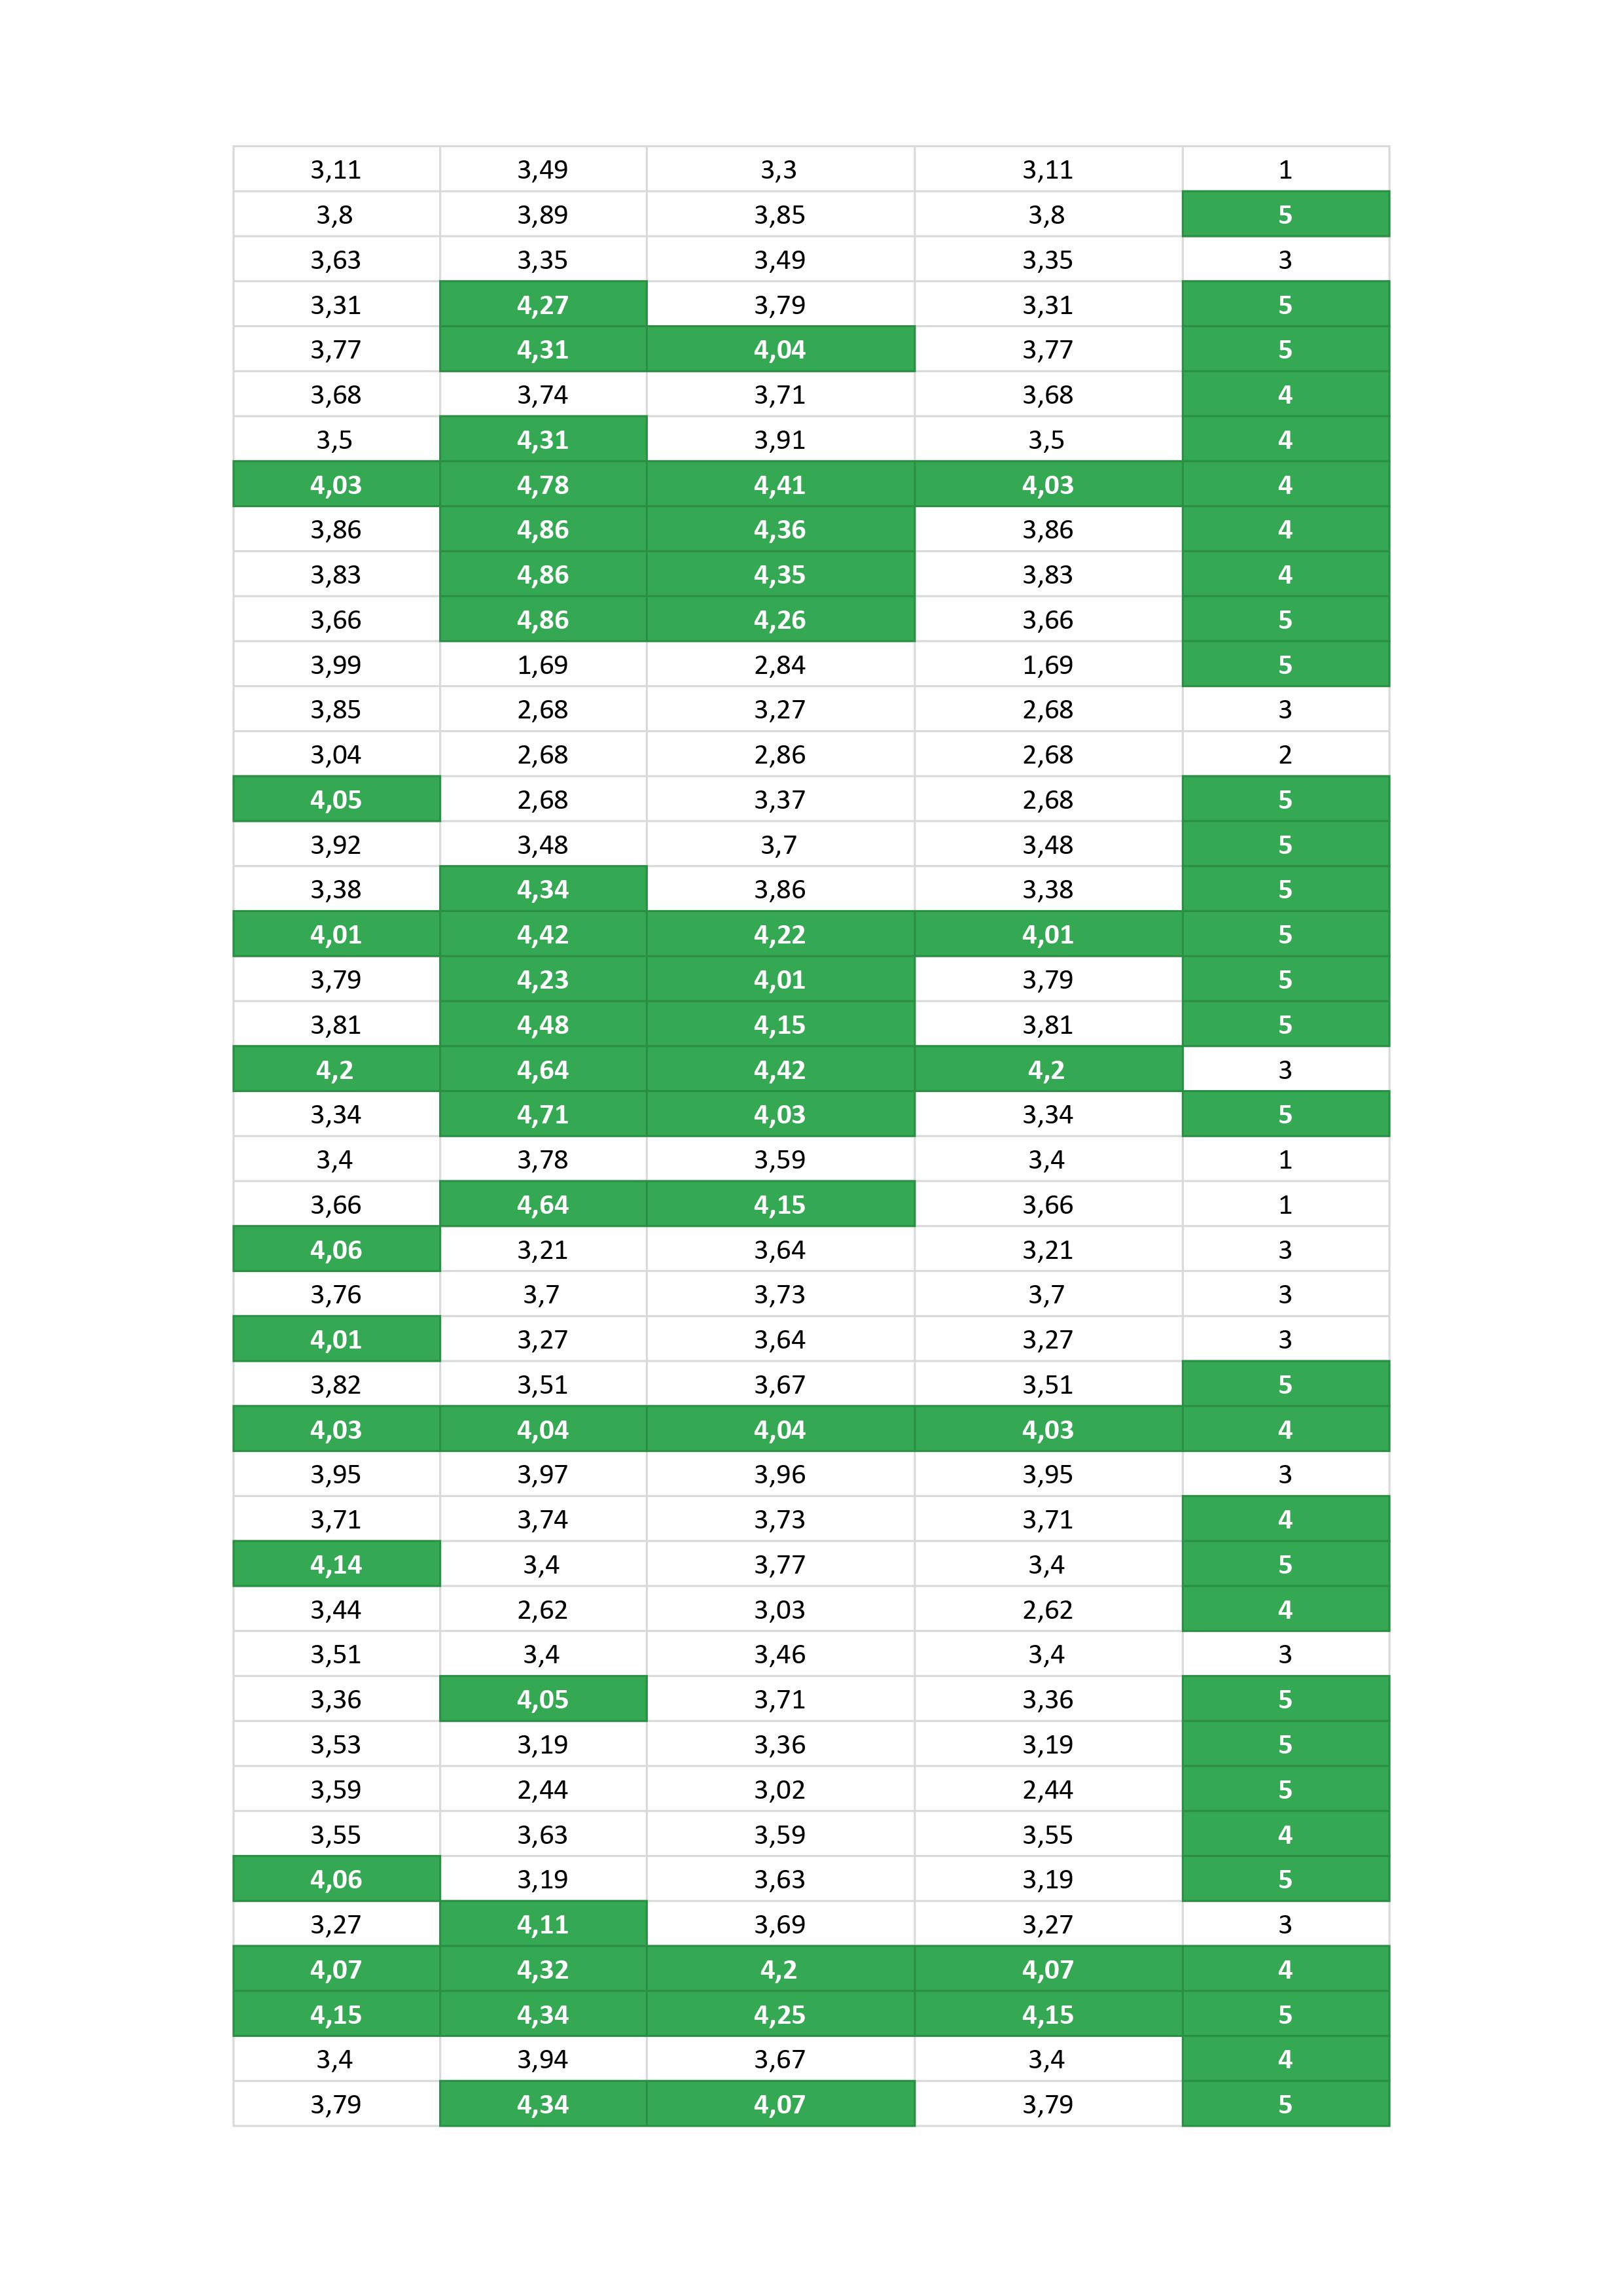
\includegraphics[width=1\linewidth]{imagens/findMusicResultados3.jpg}
	\caption[Estatística Descritiva: Parte 3]{Estatística Descritiva: Parte 3}
    \label{fig:findMusicEstatistica3}
\end{figure}

\begin{figure}[H]
	\centering
	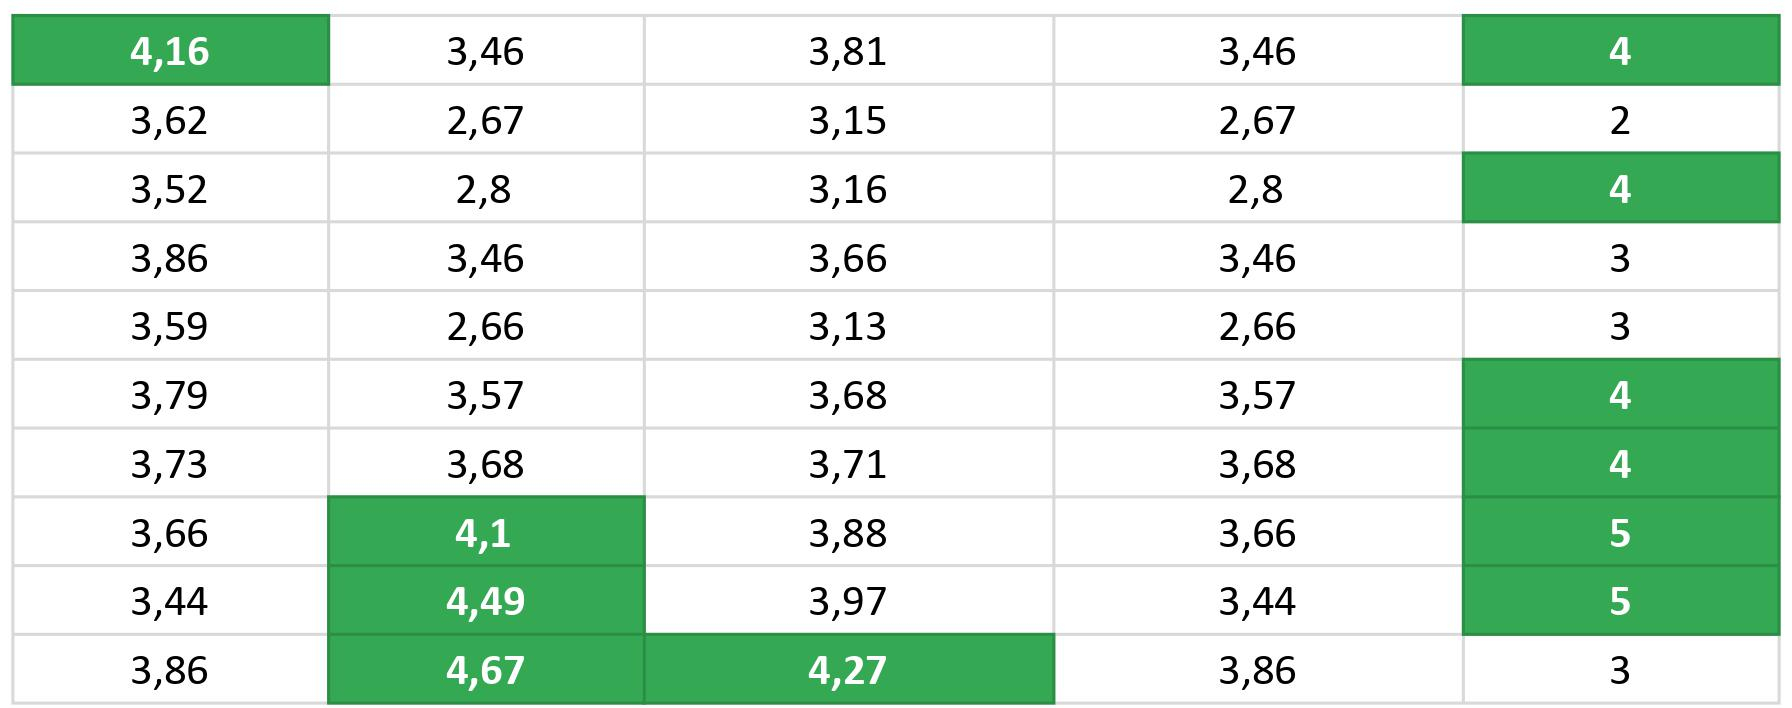
\includegraphics[width=.8\linewidth]{imagens/findMusicResultados4.jpg}
	\caption[Estatística Descritiva: Parte 4]{Estatística Descritiva: Parte 4}
    \label{fig:findMusicEstatistica4}
\end{figure}

A partir das células marcadas com a cor verde nas figuras \ref{fig:findMusicEstatistica1}, \ref{fig:findMusicEstatistica2}, \ref{fig:findMusicEstatistica3} e \ref{fig:findMusicEstatistica4}, torna-se possível observar quais itens seriam recomendados pelo sistema (tendo como consideração um ponto de corte definido como 4 pontos). Na figura \ref{fig:findMusicEstatisticaTaxa} são apresentados os resultados relativos a taxa de erros e acertos das recomendações nesse estudo de caso:

\begin{figure}[H]
	\centering
	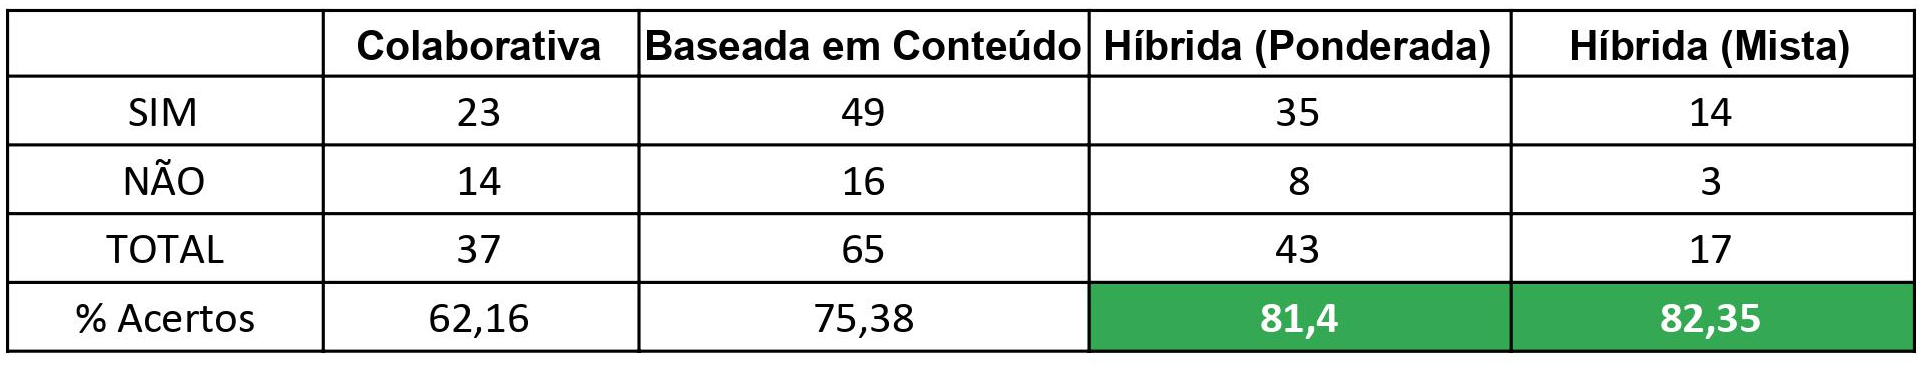
\includegraphics[width=.9\linewidth]{imagens/findmusicEstatisticaTaxa.jpg}
	\caption[Taxas da Estatística Descritiva]{Taxas da Estatística Descritiva}
    \label{fig:findMusicEstatisticaTaxa}
\end{figure}

De acordo com os dados disponíveis na figura \ref{fig:findMusicEstatisticaTaxa}, conclui-se que as abordagens híbridas (marcadas pela cor verde) obtiveram um resultado superior as estratégias colaborativa e baseada em conteúdo quando utilizadas de maneira isolada.

\subsection{Testes em T}

Como outra forma de avaliação estatística das recomendações foi utilizado o teste em T, que busca avaliar a distância entre os resultados recomendados e as notas avaliadas em determinado item pelo avaliador. Nesse tipo de abordagem é analisado a distância entre os valores recomendados e os avaliados pelos avaliadores, buscando a menor divergência entre os valores possíveis.

\begin{figure}[H]
	\centering
	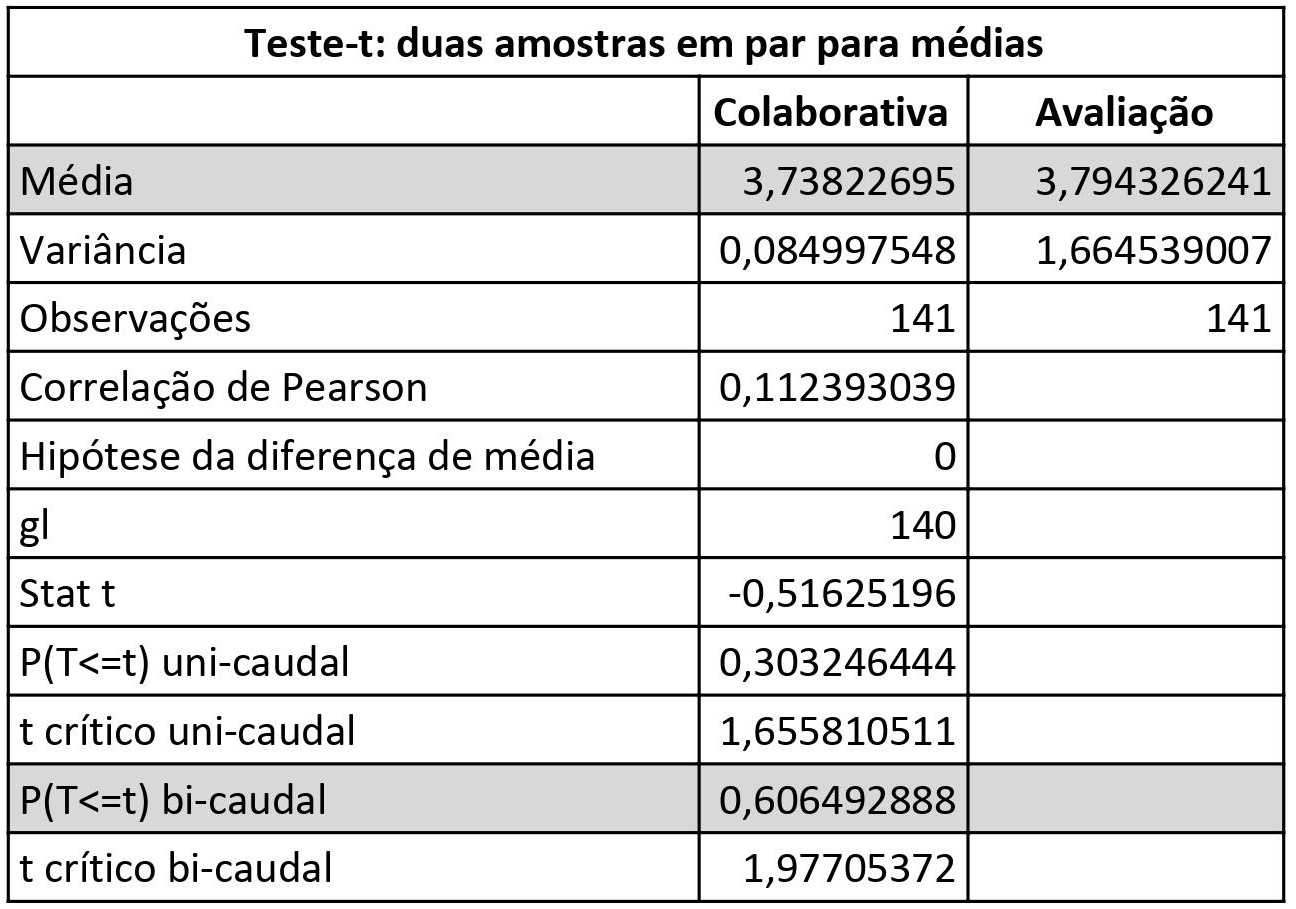
\includegraphics[width=.6\linewidth]{imagens/findmusicTesteTColaborativa.jpg}
	\caption[Teste T: Filtragem Colaborativa]{Teste T: Filtragem Colaborativa}
    \label{fig:findMusicTesteTColaborativa}
\end{figure}

A partir dos resultados obtidos na figura \ref{fig:findMusicTesteTColaborativa}, pode-se observar que o valor de \textbf{P(t<=t) bi-caudal} é superior a \textbf{0,05}. Isso significa que as recomendações para filtragem colaborativa foram boas, uma vez que apresentam similaridade com as avaliações dos usuários.

\begin{figure}[H]
	\centering
	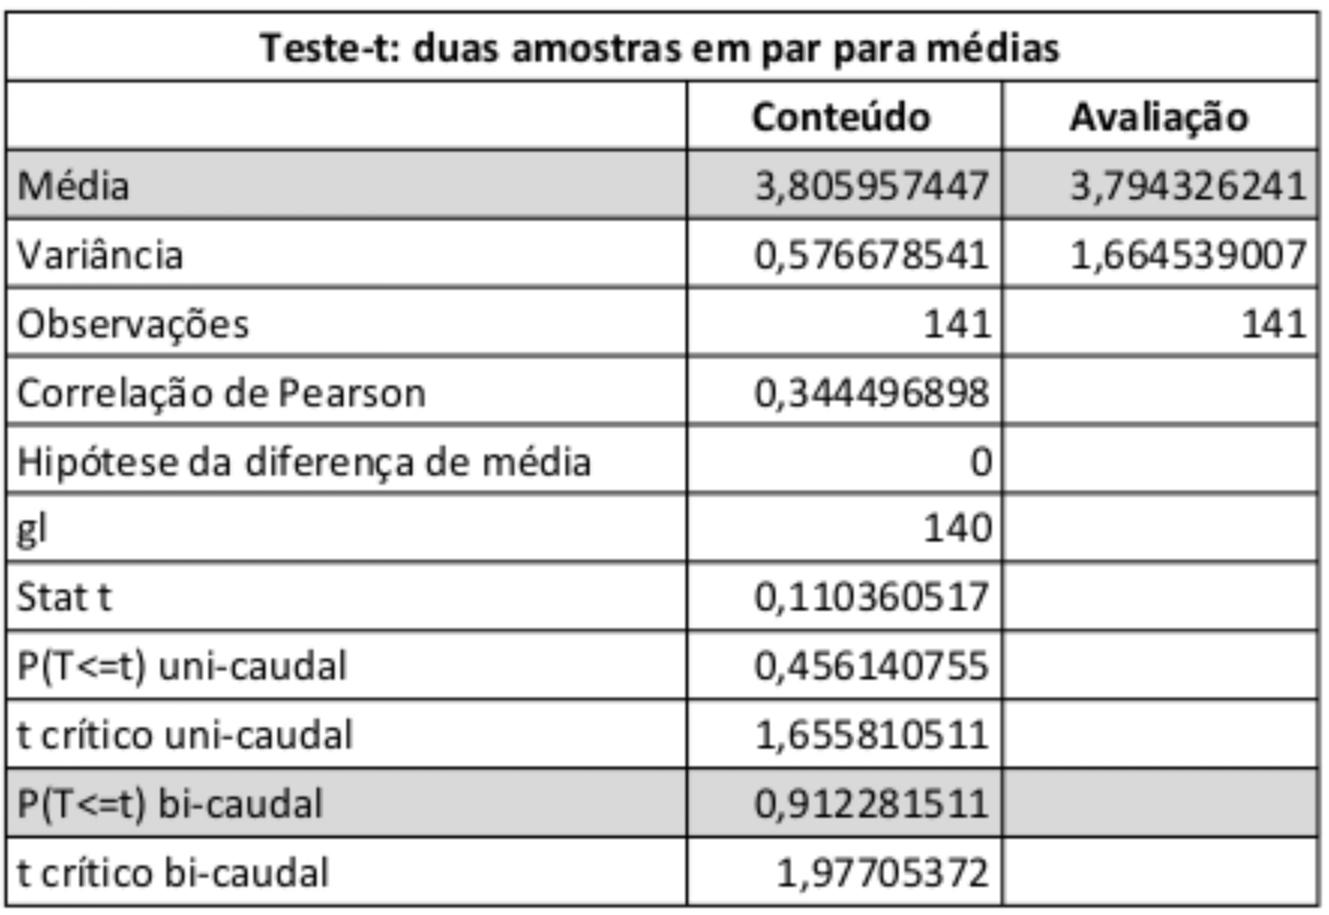
\includegraphics[width=.6\linewidth]{imagens/findmusicTesteTConteudo.jpg}
	\caption[Teste T: Filtragem Baseada em Conteúdo]{Teste T: Filtragem Baseada em Conteúdo}
    \label{fig:findMusicTesteTConteudo}
\end{figure}

A partir das informações mostradas na figura \ref{fig:findMusicTesteTConteudo}, é possível analisar que o valor \textbf{P(t<=t) bi-caudal} é superior a \textbf{0,05}. Isso demonstra que as recomendações geradas na filtragem baseada em conteúdo apresentam similaridade com as avaliações dos usuários.

\begin{figure}[H]
	\centering
	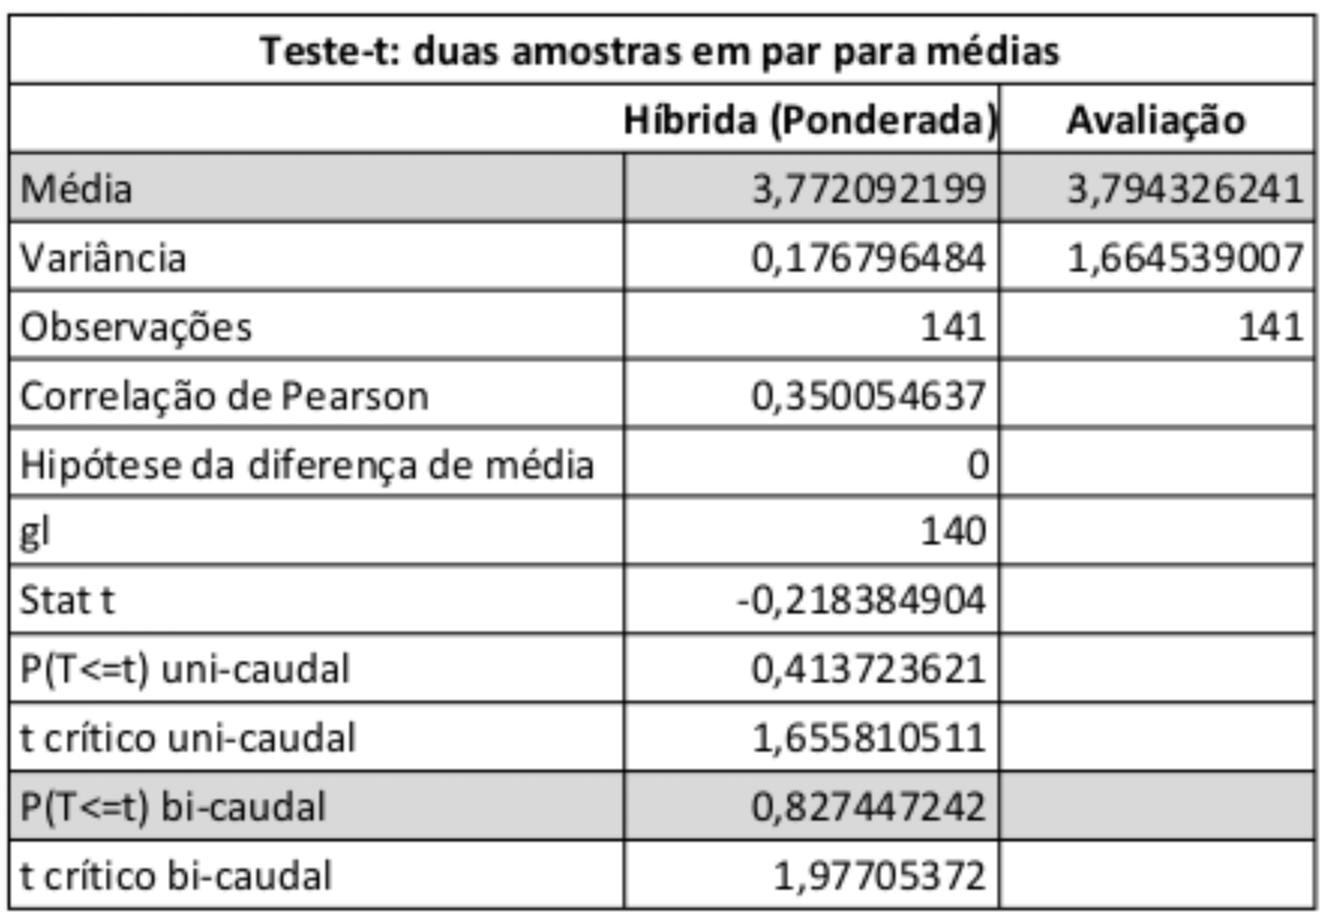
\includegraphics[width=.6\linewidth]{imagens/findmusicTesteTPonderado.jpg}
	\caption[Teste T: Filtragem Híbrida Ponderada]{Teste T: Filtragem Híbrida Ponderada}
    \label{fig:findMusicTesteTPonderado}
\end{figure}

Com os dados definidos na figura \ref{fig:findMusicTesteTPonderado}, é possível observar que o valor \textbf{P(t<=t) bi-caudal} superior a \textbf{0,05}. Isso demonstra que as recomendações da filtragem híbrida ponderada são similares as avaliações dos usuários.

\begin{figure}[H]
	\centering
	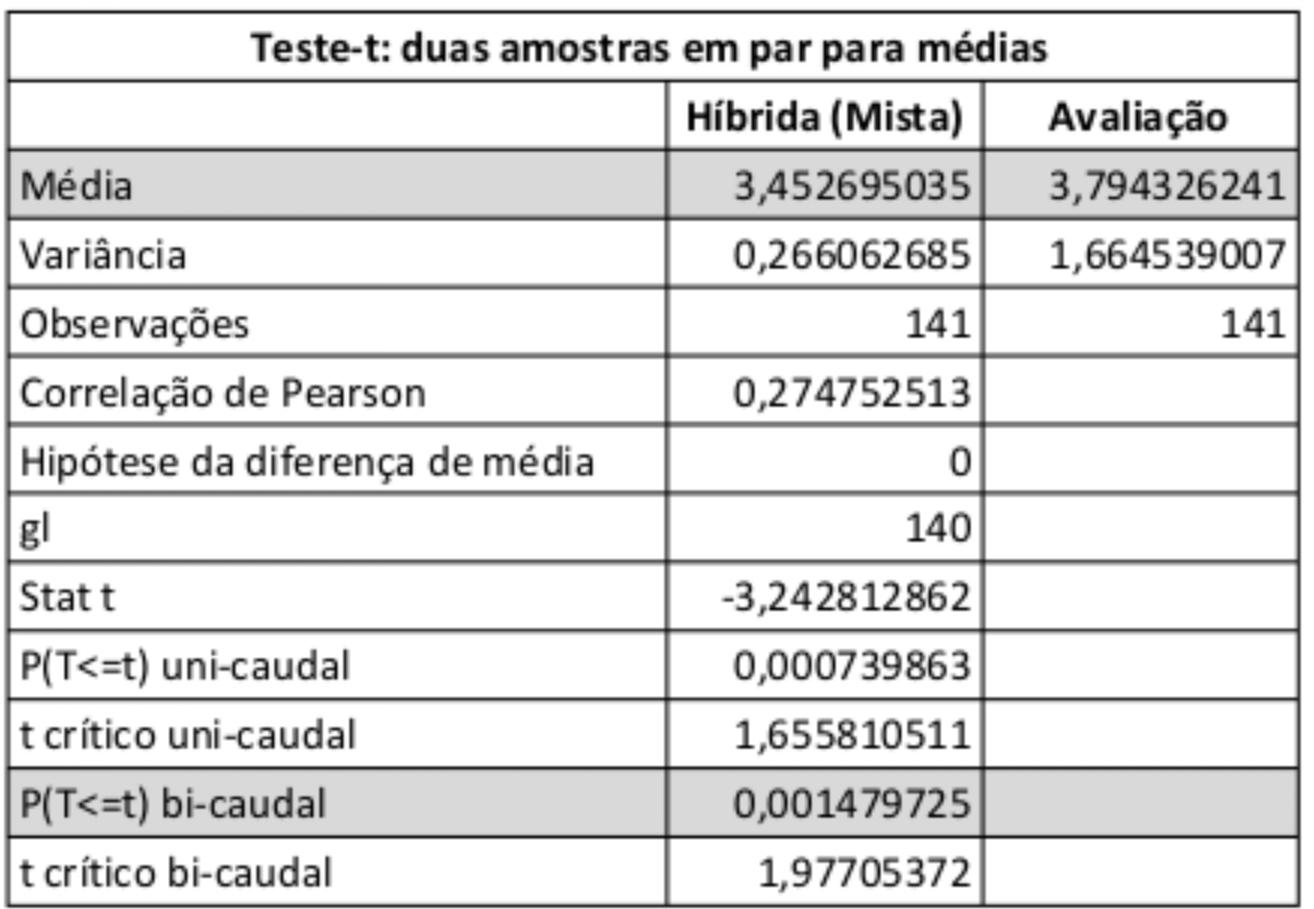
\includegraphics[width=.6\linewidth]{imagens/findmusicTesteTMista.jpg}
	\caption[Teste T: Filtragem Híbrida Mista]{Filtragem Híbrida Mista}
    \label{fig:findMusicTesteTMista}
\end{figure}

De acordo com a figura \ref{fig:findMusicTesteTMista}, os resultados das recomendações da abordagem híbrida mista não apresentam bons níveis de similaridade com as avaliações dos usuários, visto que, o valor \textbf{P(t<=t) bi-caudal} é inferior a \textbf{0,05}.